%----------------------------------------------------------------
%% Template adaptado para preparação de trabalho de conclusão de 
%% curso   (TCC)   do   Departamento   de   Economia   da 
%% Universidade      Estadual     de      Londrina       (UEL)
%
%% Autores: 
%% Prof Ph.D. Joanna G. Alexopoulos
%% Prof. Dr. Marcelo S. Bego 
%%
%% Modificações:
%% Lucas Alvarenga
%
%% Data da última atualização: 25/08/2024
%----------------------------------------------------------------
%%
%% Customizações do abnTeX2 (http://abnTeX2.googlecode.com) 
%%
%% Este trabalho pode ser distribuído e/ou modificado sob as
%% condições da Licença Pública do LaTeX Project, versão 1.3.
%% A versão desta licença pode ser encontrada em:
%%   http://www.latex-project.org/lppl.txt
%% e faz parte da versão LaTeX 01/12/2005.
%%
%% Este trabalho tem como status de manutenção LPPL como "maintained".
%% 
%% Os atuais responsáveis por esse trabalho são: 
%% Prof Ph.D. Joanna G. Alexopoulos
%% Prof. Dr. Marcelo S. Bego 
%%
%% Mais informações sobre abnTeX2 estão disponíveis em: 
%%  https://github.com/abntex/abntex2
%%
%----------------------------------------------------------------
%% Sobre a classe abntex2.cls:
%% abntex2.cls, v-1.9.5 laurocesar
%% Copyright 2012-2015 by abnTeX2 group at https://www.abntex.net.br/ 
%%
%----------------------------------------------------------------

\documentclass[12pt,oneside,a4paper,chapter=TITLE,english,brazil,sumario=abnt-6027-2012]{abntex2}

% Modo escuro %%%%
% \usepackage{xcolor}
% \pagecolor[rgb]{0.1,0.1,0.15} %black
% \color[rgb]{0.5,0.5,0.5} %grey
% %%%%%%%%%%%%%%%% 

% %%%%%%%%%%%%%%%%
% PACOTES
% %%%%%%%%%%%%%%%%

\usepackage{lmodern}			
\usepackage[T1]{fontenc}		
\usepackage[utf8]{inputenc}		
\usepackage{indentfirst}		
\usepackage[dvipsnames]{xcolor}				
\usepackage{graphicx}			
\usepackage{microtype} 
\usepackage{multicol}
\usepackage{multirow}
\usepackage{float}	
\usepackage{lipsum}				
\usepackage{tikz}
\usepackage{ragged2e} 
\usepackage[brazilian,hyperpageref]{backref}	
\usepackage[alf]{abntex2cite}
\usepackage{blindtext} 
\usepackage{mathptmx}
\usepackage[labelfont=bf]{caption}
\captionsetup{labelfont=bf}
\usepackage[singlelinecheck=false]{caption}
\usepackage{amsmath}
\usepackage[table]{xcolor} % Para colorir tabelas
\usepackage{zref-totpages}
\usepackage{titlesec}


% %%%%%%%%%%%%%%%%
%MARGENS
%As margens são configuradas conforme a NBR 14724:2011
%As margens devem ser: para o anverso, esquerda e superior de 3 cm e direita e inferior de 2 cm; para o verso, direita e superior de 3 cm e esquerda e inferior de 2 cm.

% %%%%%%%%%%%%%%%%
%FONTES 
% %%%%%%%%%%%%%%%%

% %%%%%%%%%%%%%%%%
%TIPO DE FONTE
\renewcommand{\sfdefault}{\rmdefault} % Fonte: Times New Roman

% %%%%%%%%%%%%%%%%
% TAMANHO E ESTILO DAS FONTES DOS TÍTULOS E SUBSEÇÕES 
\renewcommand{\ABNTEXchapterfontsize}{\large \bfseries}%14pt

\renewcommand{\ABNTEXsectionfont}{\bfseries}%Subseções em negrito.

\definecolor{verdeUEL}{RGB}{10,128,20}


\setlength\afterchapskip{18pt}

% %%%%%%%%%%%%%%%%
% ESPAÇAMENTOS
% %%%%%%%%%%%%%%%%

% TAMANHO DO PARÁGRAFO 
\setlength{\parindent}{1.27cm} %Primeira linha

%ESPAÇO ENTRE LINHAS
%O padrão é definido como \OnehalfSpacing (1.5)


% %%%%%%%%%%%%%%%%
%INFORMAÇÕES DA CAPA, FOLHA DE ROSTO E FOLHA DE APROVAÇÃO 
% %%%%%%%%%%%%%%%%

% %%%%%%%%%%%%%%%%
%NOME DO TRABALHO 
\titulo{\bfseries ANÁLISE DA DINÂMICA INFLACIONÁRIA SOB O REGIME DE METAS DE INFLAÇÃO NO BRASIL ENTRE 2003 e 2023}


% %%%%%%%%%%%%%%%%
%NOME DO AUTOR 
\autor{LUCAS BONI DOS ANJOS AMARAL ALVARENGA}


% %%%%%%%%%%%%%%%%
%NOME DO ORIENTADOR
\orientador{Carlos Eduardo Caldarelli}


% %%%%%%%%%%%%%%%%
\local{Londrina}
\data{\the\year}
\tipotrabalho{monografia}
\instituicao{Universidade Estadual de Londrina (UEL)}
\preambulo{Trabalho de Conclusão de Curso apresentado ao Departamento de Economia da Universidade  Estadual de Londrina.}
% %%%%%%%%%%%%%%%%


% %%%%%%%%%%%%%%%%
% CAPA UEL
\renewcommand{\imprimircapa}{
	\begin{capa}
		\center
		\begin{figure}
		
\includegraphics[height=3.65cm,width=15.5cm]{fig/Logo_UEL_new.png}
		\end{figure}

		% \begin{tikzpicture}
		% \fill[verdeUEL] (17.1,1.25) rectangle (1,1);
		% \end{tikzpicture}
		% \large 
		
		{\bfseries CENTRO DE ESTUDOS SOCIAIS APLICADOS\\
		DEPARTAMENTO DE ECONOMIA\\
		CURSO DE CIÊNCIAS ECONÔMICAS\\}
		
		
		\vspace{5cm}
		
		{\ABNTEXchapterfont\textsc{\Large\imprimirtitulo}}
		
		\vfill
		
		\begin{flushright}
			\imprimirautor
			\vspace{-0.5cm}
			
		\end{flushright}
		
		\begin{tikzpicture}
		\fill[verdeUEL] (17.1,1.125) rectangle (1,1);
		\end{tikzpicture}
		
		{\imprimirlocal}
		
		{\imprimirdata}
		
	\end{capa}
}


\emergencystretch 3em
\hyphenpenalty 10000
\exhyphenpenalty 10000

% %%%%%%%%%%%%%%%%
% FOLHA DE ROSTO
\makeatletter

\renewcommand{\folhaderostocontent}{
	\begin{center}
      \large 	
	
	  {\ABNTEXchapterfont\textsc{\Large \imprimirautor}}
		
		\vspace{6cm}
		
		{\ABNTEXchapterfont\textsc{\Large \imprimirtitulo}}
		
		\vspace{2cm}
		
		\begin{flushright}
			\begin{minipage}{8cm}
				\SingleSpacing

				Trabalho de Conclusão de Curso apresentado à Universidade Estadual de Londrina - UEL, como requisito parcial para a obtenção do título de Bacharel em Ciências Econômicas.
				\break
				
				Orientador: Prof. Dr. \imprimirorientador
			\end{minipage}%
		\end{flushright}
		
		\vfill
		
		
		{\large\imprimirlocal}
		
		{\large\imprimirdata}
	\end{center}
}
\makeatother


% %%%%%%%%%%%%%%%%
% FOLHA DE APROVAÇÃO 
\makeatother

\newcommand{\folhaDeaprovacao}{
	\begin{center}
		
		\begin{folhadeaprovacao} 
			\begin{center} 
				
					
				
			{\ABNTEXchapterfont\textsc{\large \imprimirautor}}
				
				\vspace{2cm}
				
			{\ABNTEXchapterfont\textsc{\large \imprimirtitulo}}
				
				\vspace{1cm}		
				\begin{flushright}
					\begin{minipage}{10cm}
						\SingleSpacing
						Trabalho de Conclusão de Curso apresentado à Universidade Estadual de Londrina - UEL, como requisito parcial para a obtenção do título de Bacharel em Ciências Econômicas.
					\end{minipage}%
				\end{flushright}	
				
				\vspace{2cm}
				
				\begin{flushright}
					\begin{minipage}{10cm}		
						\centering
					{\bfseries COMISSÃO EXAMINADORA}
					\end{minipage}
				\end{flushright}	
				
				\vspace{1cm}
				
				\begin{flushright}
					\begin{minipage}{10cm}	
						\centering
						\hrule \hspace{0.2cm}
						
						Orientador(a): Prof(a). \imprimirorientador  
						
						\imprimirinstituicao
					\end{minipage}%
				\end{flushright}
				
				\vspace{1cm}
				
				\begin{flushright}
					\begin{minipage}{10cm}	
						\centering
						\hrule \hspace{0.2cm}
						
						Prof(a). NOME BANCA 1
						
						\imprimirinstituicao
					\end{minipage}%
				\end{flushright}		
				
				
				\vspace{1cm}
				
				\begin{flushright}
					\begin{minipage}{10cm}	
						\centering
						\hrule \hspace{0.2cm}
						
						Prof(a). NOME BANCA 2 
						
						\imprimirinstituicao
					\end{minipage}%
				\end{flushright}
				
				\vfill 
				
				\begin{flushright}
					\begin{minipage}{6cm}	
				\centering
				Londrina, 27 de Agosto de \imprimirdata.
					\end{minipage}
			\end{flushright}
		
			\end{center} 
		\end{folhadeaprovacao}
	\end{center}
}
\makeatother


% %%%%%%%%%%%%%%%%
%REGULAMENTO DO TRABALHO DE CONCLUSÃO DO CURSO DE ECONOMIA (DISCIPLINAS MONOGRAFIA I E II - 6TCC404 E 6TCC405)
% %%%%%%%%%%%%%%%%

%ART.16 A estrutura da monografia compõe-se de:

%I. Capa;
%II. Folha de rosto;
%III. Elementos pré-textuais;
%IV. Resumo e “Abstract” (ou versão em Espanhol ou ainda em Francês):
%V. Sumário;
%VI. Introdução;
%VII. Desenvolvimento, contendo Referencial Teórico ou Econométrico ou Revisão de Literatura ou Revisão Bibliográfica ou Modelo Teórico; e nos casos de estudos quantitativos Metodologia e Fonte e tratamento de dados;
%VIII. Resultados e discussão;
%IX. Considerações finais ou Conclusão;
%X. Referências;
%XI. Anexos e Apêndices, quando for o caso
%%%%%%%%%%%%%%%%%%%%%%%%%%%%



% INÍCIO DO DOCUMENTO
\begin{document}

% Retira espaço extra obsoleto entre as frases.
\frenchspacing 


% %%%%%%%%%%%%%%%%
% CAPA
\imprimircapa

% %%%%%%%%%%%%%%%%
%FOLHA DE ROSTO
\folhaderostocontent


% %%%%%%%%%%%%%%%%
%FIXA CATALOGRÁFICA 
%Incluir fica catalográfica
%\pagebreak


% %%%%%%%%%%%%%%%%
%FOLHA DE APROVAÇÃO 
\folhaDeaprovacao


% %%%%%%%%%%%%%%%%
%DEDICATÓRIA
\begin{dedicatoria}
	\vspace*{\fill}
	\noindent
	Dedico esse trabalho aos meus pais, Bruno e Silvia, por todo amor, apoio e incentivo, que foram fundamentais para a realização de mais uma conquista. Sua dedicação e sacrifícios me proporcionaram a oportunidade de realizar meus sonhos.
	\vspace*{\fill}
\end{dedicatoria}


% %%%%%%%%%%%%%%%%
%AGRADECIMENTOS
\begin{agradecimentos}
	\noindent
	Agradeço ao meu orientador, Prof. Dr. Carlos Eduardo Caldarelli, por toda ajuda, conhecimento e experiência que compartilhou comigo durante a confecção desse trabalho.
	Agradeço a todos meus professores e a todos os meus colegas de curso, que contribuíram com conhecimentos, experiências e incentivos, tornando minha jornada mais rica e gratificante. Aos amigos, que estiveram presentes nos momentos de lazer e de estudo, proporcionando equilíbrio e motivação durante o percurso.	À Universidade Estadual de Londrina por oferecer um ambiente de aprendizado e crescimento tão acolhedor. A todos aqueles que, direta ou indiretamente, colaboraram para a conclusão deste trabalho.
\end{agradecimentos}


% %%%%%%%%%%%%%%%%
%RESUMO

\setlength{\absparsep}{18pt} % ajusta o espaçamento dos parágrafos do resumo
\begin{resumo}

	\noindent
	ALVARENGA, Lucas. {\bfseries Análise da Dinâmica Inflacionária Sob o Regime de Metas de Inflação no Brasil Entre 2003 e 2023}. \imprimirdata. \ztotpages \, f. Monografia (Graduação em Ciências Econômicas). Centro de Estudos Sociais Aplicados, Universidade Estadual de Londrina, Londrina, 2024.
	
	Este trabalho tem por objetivo verificar o impacto da inflação, principalmente sob a ótica da oferta e da demanda sobre a economia brasileira e avaliar os efeitos exercidos por estas sobre a eficácia do regime de metas de inflação (RMI) no Brasil. Será examinado se as respostas do Banco Central são eficientes e sob quais óticas a política monetária deve ser definida a fim de atender os objetivos propostos pelo RMI. Por meio deste trabalho, busca-se atingir um melhor entendimento dos mecanismos que regem a dinâmica inflacionária no Brasil e como é moldada a resposta à inflação pela autoridade monetária brasileira. Para isso, será utilizado o modelo econométrico de vetores autorregressivos (VAR), que consegue capturar relações de longo prazo entre as variáveis escolhidas, que são a meta de inflação anual do Banco Central, a taxa de câmbio entre o Real e o Dólar Americano, o produto interno bruto (PIB) real do Brasil, o Índice Nacional de Preços ao Consumidor Amplo (IPCA) e o Índice de Preços ao Produtor Amplo, Estágios de Produção - Disponibilidade Interna (IPA-EP-DI).
	
	\textbf{Palavras-chave}: inflação; oferta; demanda; econometria; política monetária.
\end{resumo}


% %%%%%%%%%%%%%%%%
%ABSTRACT
% \noindent
% ALVARENGA, Lucas. {\bfseries Análise da Dinâmica Inflacionária Sob o Regime de Metas de Inflação no Brasil Entre 2003 e 2023}, \imprimirdata. <FOLHAS> f. Monografia (Curso de Ciências Econômicas). Centro de Estudos Sociais Aplicados, Universidade Estadual de Londrina, Londrina, 2024.

% \begin{resumo}[Abstract]
% 	\begin{otherlanguage*}{english}

% 		Write your abstract here... 

% 		\vspace{\onelineskip}

% 		\noindent 
% 		\textbf{Keywords}: 
% 	\end{otherlanguage*}
% \end{resumo}
% \pagebreak


% %%%%%%%%%%%%%%%%
%LISTA DE FIGURAS
\pdfbookmark[0]{\listfigurename}{lof}
\listoffigures*
\cleardoublepage


% %%%%%%%%%%%%%%%%
%LISTA DE TABELAS
\pdfbookmark[0]{\listtablename}{lot}
\listoftables*
\cleardoublepage


% %%%%%%%%%%%%%%%%
%LISTA DE ABREVIATURAS
\begin{siglas}
	\item[UEL] Universidade Estadual de Londrina. 
	\item[ABNT] Associação Brasileira de Normas Técnicas.
	\item[RMI] Regime de metas de inflação
	\item[SELIC] Sistema Especial de Liquidação e Custódia
	\item[IPA-EP-DI] Índice de Preços ao Produtor Amplo, Estágios de Produção, Disponibilidade Interna
	\item[IPCA] Índice Nacional de Preços ao Consumidor Amplo
	\item[IBGE] Instituto Brasileiro de Geografia e Estatística
	\item[IGP-DI] Índice Geral de Preços - Disponibilidade Interna
	\item[CMN] Conselho Monetário Nacional
	\item[ECM] Modelagem de Correção de Erros
	\item[VAR] Análise de Vetores Autoregressivos
	\item[PIB] Produto Interno Bruto
	\item[PAI] Programa de Ação Imediata
	\item[PEC] Proposta de Emenda à Constituição
	\item[BCB] Banco Central do Brasil
	\item[IPP] Índice de Preços ao Produtor
	\item[MQO] Método de Mínimos Quadrados Ordinários
	\item[MQG] Método de Mínimos Quadrados Generalizados
	\item[ADF] Teste de Dickey-Fuller Aumentado
	\item[PP] Teste de Phillips-Perron
	\item[IRF] Função de Impulso-Resposta
	\item[VD]  Decomposição de Variância
	\item[AIC] Critério de Informação de Akaike
	\item[BIC] Critério de Informação Bayesiano
	\item[IPEA] Instituto de Pesquisa Econômica Aplicada
\end{siglas}
\pagebreak


% %%%%%%%%%%%%%%%%
%LISTA DE SíMBOLOS
% \begin{simbolos}
% 	\item[Depeco] Departamento de Economia
% \end{simbolos}
% \pagebreak


% %%%%%%%%%%%%%%%%
% SUMÁRIO
\pdfbookmark[0]{\contentsname}{toc}
\tableofcontents*
\cleardoublepage


% %%%%%%%%%%%%%%%%
%INÍCIO DO TEXTO
\textual % indica o início do texto para a numeração das páginas
\pagestyle{simple}
\aliaspagestyle{chapter}{simple}

\chapter{Introdução}

O controle da inflação é um dos principais desafios enfrentados pelas autoridades econômicas em diversas nações ao redor do mundo. No Brasil, a adoção do Regime de Metas de Inflação (RMI) em 1999 representou uma mudança significativa na condução da política monetária, com o objetivo de estabilizar os preços e promover um ambiente econômico previsível \cite{fraga_2003_inflation}. Diante desse contexto, este trabalho tem como objetivo analisar a dinâmica inflacionária no Brasil sob o RMI entre os anos de 2003 e 2023, focando especificamente nos componentes de inflação de demanda e de oferta para verificar a efetividade das políticas do Banco Central.

Ao longo deste trabalho, serão abordados os diferentes tipos de inflação, seguido por um detalhamento do histórico econômico brasileiro e uma discussão sobre o RMI e a política monetária na terceira seção. A quarta seção detalhará a metodologia, os modelos utilizados e os dados coletados. Os resultados e sua subsequente discussão serão apresentados na quinta seção, culminando com a conclusão na sexta seção. Por meio desta análise, espera-se contribuir para uma melhor compreensão da dinâmica inflacionária no Brasil e a eficácia do RMI na promoção da estabilidade econômica, assim como os impactos sobre o produto e o desenvolvimento econômico.

Para compreender o cenário a ser estudado, definimos o Regime de Metas de Inflação como um arranjo institucional em que o Banco Central se compromete a manter a inflação dentro de um intervalo preestabelecido, utilizando instrumentos de política monetária, como as operações em \textit{open market}, para alcançar esse objetivo \cite{svensson_1997_inflation}. Este regime busca ancorar as expectativas inflacionárias dos agentes econômicos, contribuindo para a estabilidade macroeconômica \cite{mishkin_2000_inflation}. Desde sua implementação, o RMI no Brasil tem se baseado em metas anuais de inflação definidas pelo Conselho Monetário Nacional (CMN), com o Banco Central ajustando a taxa do Sistema Especial de Liquidação e Custódia (SELIC) via instrumentos de política monetária para controlar a demanda agregada e manter a inflação dentro dos limites estipulados.

De acordo com o Banco Central do Brasil (2013), A taxa SELIC é obtida através do cálculo da taxa média ponderada e ajustada das operações de financiamento de um dia, que são garantidas por títulos públicos federais. Essas operações ocorrem no sistema financeiro ou em câmaras de compensação e liquidação de ativos, sob a forma de operações compromissadas, onde o vendedor se compromete a recomprar os títulos vendidos no dia útil seguinte. Abaixo, na equação 1.1, é dada a fórmula utilizada para o cálculo da taxa:

\begin{equation}
	\left[ \left( \left(\frac{\sum_{j=1}^{n} L_j \cdot V_j}{\sum_{j=1}^{n} V_j} \right)^{252} - 1 \right) \times 100 \right] \textrm{\% ao ano}
\end{equation}


A equação 1.1 baseia-se em três principais variáveis, sendo elas $L_j$, o fator diário correspondente à taxa da j-ésima operação, $V_j$, o valor financeiro correspondente à taxa da j-ésima operação e $n$, o número de operações que compõem a amostra. A taxa SELIC é principalmente ajustada pelas operações de mercado aberto (\textit{open market}), instrumento da política monetária onde o Banco Central realiza a compra ou venda de títulos da dívida pública aos principais bancos comerciais brasileiros.

Considerando o que foi exposto acima, temos que o ajuste da da taxa SELIC reflete os movimentos do Banco Central no controle da inflação ao influenciar a oferta de moeda e o custo do crédito no mercado. A variação na taxa básica de juros, promovida pelas operações de mercado aberto, tem, portanto, efeitos diretos sobre os níveis de consumo e investimento na economia. A política monetária, ao atuar na direção de modificar a taxa SELIC, busca equilibrar o crescimento econômico com as pressões inflacionárias, que podem ter diferentes origens e dinâmicas.

Assim, detalhamos os diferentes tipos de inflação experienciados pelo país para analisar como o Banco Central tem respondido às mudanças nas variáveis macroeconômicas. A economia brasileira, como muitas outras, está sujeita a um descompasso entre o crescimento econômico real e a base monetária, resultando em inflação. O processo inflacionário pode ter como fonte diversos fatores, sendo comum verificar a inflação de oferta, a inflação de demanda, a inflação inercial e a inflação estrutural. Cada um desses tipos de inflação apresenta características distintas que influenciam a eficácia do RMI, como será observado ao decorrer deste trabalho.

Como exemplo, a inflação de oferta é impulsionada por choques nos custos de produção, como aumentos nos preços de matérias-primas ou salários \cite{blinder_2008_the}. Aumentar a taxa de juros em resposta a esse tipo de inflação pode, porém, ser ineficaz, uma vez que abre oportunidade para o resfriamento da economia, já que não combate a causa raiz do processo inflacionário para esse caso em particular. Compreender a interação entre os tipos de inflação e o funcionamento do RMI é crucial para avaliar a eficácia das políticas monetárias adotadas pelo Banco Central do Brasil nas últimas décadas. Nesse contexto, o presente trabalho pretende investigar como a inflação de demanda e de oferta influenciaram a dinâmica inflacionária no Brasil durante o período analisado e como o RMI respondeu a esses desafios.

Para isso, são utilizadas técnicas econométricas aplicadas a séries temporais relacionadas aos índices de preços, tanto pelo lado da oferta, com indicadores como o  Índice de Preços ao Produtor Amplo (Disponibilidade Interna) (IPA-EP-DI), quanto pelo lado de demanda, com indicadores como o IPCA (Índice de Preços ao Consumidor Amplo). Também são utilizados outros indicadores macroeconômicos pertinentes, como o produto interno bruto (PIB) e a taxa de câmbio entre o Real brasilero e o Dólar Estadunidense.

A análise de séries temporais permite modelar e prever o comportamento de variáveis econômicas ao longo do tempo, capturando tanto as tendências quanto as flutuações cíclicas e sazonais \cite{enders_2015_applied}. Métodos como a Análise de Vetores Autoregressivos (VAR), a Modelagem de Correção de Erros (ECM) e os testes de raiz unitária são frequentemente utilizados para investigar a relação entre a política monetária e a inflação \cite{hamilton_2020_time}.

A aplicação de econometria a séries temporais envolve várias etapas, incluindo a identificação e a modelagem das propriedades estocásticas das séries de dados, a estimação dos parâmetros do modelo e a realização de testes de hipóteses para validar os resultados \cite{stock_2020_introduction}. Essas técnicas nos permite avaliar a resposta da inflação a choques de demanda e oferta, bem como a eficácia das intervenções do Banco Central no controle dos preços. A seguir, iniciamos pela descrição aprofundada dos tipos de inflação que a economia brasileira observou historicamente e sua relação com o RMI.

\chapter{Tipos de Inflação}

Historicamente, o Brasil enfrentou diferentes tipos de inflação, cada um decorrente de fatores econômicos e contextos específicos. Nos anos de 1980 e início dos anos 1990, por exemplo, o país sofreu com altos níveis de inflação, caracterizada por aumentos de preços extremamente rápidos e incontroláveis. Esse período foi marcado por políticas econômicas instáveis, déficits fiscais elevados e um ciclo de indexação de preços, onde os preços e salários eram ajustados automaticamente à inflação passada, perpetuando o ciclo inflacionário. Para \citeonline{bresser_1990_hiperinfla}, o fator desencadeante da hiperinflação foi a crise fiscal dos anos 1980, que pode ser desmembrada em três elementos: o déficit público, a dívida pública, tanto interna quanto externa, e o curto prazo de vencimento dos títulos públicos.

% TODO: citation to back this up? https://www.scielo.br/j/rec/a/4ZqfqsrqsHwFJV9QjJWYsfN/?lang=pt

O Brasil experenciou de forma ostensiva a inflação inercial no final do século XX. Esse fenômeno é como um ciclo vicioso, uma vez que a inflação persiste devido à expectativa de que ela continuará, independentemente de outros fatores econômicos. Nos anos 1990, especialmente antes do Plano Real, a inflação inercial era alimentada pela indexação, onde preços e contratos eram ajustados automaticamente com base na inflação passada. O Plano Real, implementado em 1994, conseguiu quebrar essa inércia ao introduzir uma nova moeda e uma série de reformas econômicas que estabilizaram a economia. A partir desse ponto, o Brasil passou a experimentar uma inflação mais controlada, embora ainda enfrentasse desafios ocasionais devido a choques externos e flutuações internas na economia.

Abaixo, na Tabela \ref{table:currencyhist}, é apresentado um breve histórico das moedas que circularam na economia brasileira. É interessante observar como a base monetária se expandiu ao longo do tempo, principalmente a partir do Cruzeiro na década de 1970, momento em que houve sucessivos "cortes de zero", onde a nova moeda possuia valores nas cédulas geralmente mil vezes menores do que a moeda anterior.

\vspace{0.2cm}

\begin{table}[H]
	\caption{Histórico de moedas brasileiras}
	\centering
	\rowcolors{2}{gray!8}{white}
	\begin{tabular}{ | l || c | l | }
		\hline
		\textbf{Moeda Vigente}                      & \textbf{Período de Vigência} & \textbf{Equivalência}      \\
		\hline
		\textbf{Cruzeiro}                           & 1942 a 1964                  & Cr\$ 1,00 = Rs 1\$000      \\
		\textbf{Cruzeiro (retirada dos centavos)}   & 1964 a 1967                  & Cr\$ 1 = Cr\$ 1,00         \\
		\textbf{Cruzeiro Novo (volta dos centavos)} & 1967 a 1970                  & NCr\$ 1,00 = Cr\$ 1.000    \\
		\textbf{Cruzeiro}                           & 1970 a 1984                  & Cr\$ 1,00 = NCr\$ 1,00     \\
		\textbf{Cruzeiro (retirada dos centavos)}   & 1984 a 1986                  & Cr\$ 1 = Cr\$ 1,00         \\
		\textbf{Cruzado (volta dos centavos)}       & 1986 a 1989                  & Cz\$ 1,00 = Cr\$ 1.000     \\
		\textbf{Cruzado Novo}                       & 1989 a 1990                  & NCz\$ 1,00 = Cz\$ 1.000,00 \\
		\textbf{Cruzeiro}                           & 1990 a 1993                  & Cr\$ 1,00 = NCz\$ 1,00     \\
		\textbf{Cruzeiro Real}                      & 1993 a 1994                  & CR\$ 1,00 = Cr\$ 1.000,00  \\
		\textbf{Real}                               & Desde 1994                   & R\$ 1,00 = CR\$ 2.750,00   \\                                                                  
		\hline
	\end{tabular}
	
	\label{table:currencyhist}
	\vspace{1ex}
	
	\raggedright{
		\noindent \footnotesize{Fonte: Histórico das Alterações da Moeda Nacional. Disponível em \\ https://web.archive.org/web/20151115205007/http://www.ocaixa.com.br/passos/passos2.htm.}}
\end{table}
\vspace{-0.2cm}
\vspace{0.5cm}

Desde o Cruzeiro, passando pelo Cruzado, até chegar ao Real, cada uma das moedas observadas na Tabela \ref{table:currencyhist} surgiu em resposta a crises inflacionárias e à perda de confiança na moeda nacional vigente na época. Essas mudanças foram frequentemente catalisadas por eventos externos, como crises internacionais, choques no preço do petróleo, e também por fatores internos, como descontrole fiscal e políticas econômicas inconsistentes. Abaixo, detalhamos como a instabilidade econômica, que impacta diretamente a capacidade produtiva das empresas e o custo dos produtos e serviços, contribui para a inflação de oferta.

\section{Inflação de Oferta}

Um exemplo marcante de inflação de oferta, tanto no Brasil quanto no mundo, ocorreu durante as crises do petróleo dos anos 1970. O aumento abrupto dos preços do petróleo, um insumo fundamental para diversas indústrias, resultou em custos mais altos de transporte e produção, impactando a economia brasileira. Outro exemplo mais recente foi observado durante a crise hídrica na região sudeste em 2014 e 2015, quando a escassez de água afetou a produção agrícola e a geração de energia hidrelétrica, levando ao aumento dos custos de alimentos e eletricidade (FRANCO, 2014).

É também conhecida como inflação de custos e ocorre quando os custos de produção aumentam, levando a um aumento nos preços dos bens e serviços finais. Esses aumentos nos custos podem ser decorrentes de elevações nos preços das matérias-primas, aumentos salariais, ou choques de oferta adversos, como desastres naturais ou interrupções no fornecimento de insumos essenciais. \citeonline{blinder_2008_the} descrevem a inflação de custos como um fenômeno onde os produtores, enfrentando maiores custos de produção, repassam esses custos para os consumidores através de preços mais altos.

"A inflação de custos, além de elevar o nível de preços da economia, causa estagflação, expressão empregada quando a economia apresenta alto nível de preços e contração do produto interno bruto, diferentemente da inflação de demanda, onde a expansão da demanda agregada, além de elevar o nível de preços, aquece a economia e estimula o crescimento do PIB" \cite{cortapasso_estagflacao}.

Logo, combater a inflação de oferta envolve várias estratégias, incluindo a melhoria da infraestrutura para reduzir custos de produção e distribuição, a diversificação de fontes de insumos para diminuir a dependência de um único fornecedor e o incentivo à inovação e adoção de novas tecnologias para aumentar a produtividade. Além disso, políticas cambiais que estabilizem a moeda podem minimizar os impactos de variações cambiais nos custos de insumos importados. 

Visto que o principal canal de transmissão da política monetária exercitado pelo Banco Central do Brasil (BCB) não é o cambial, mas sim a taxa SELIC, em um caso de inflação de custos, a principal resposta seria a modificação da taxa de juros básica da economia. Um aumento da taxa de juros em resposta a esse tipo de inflação, porém, pode ser ineficaz ou até prejudicial, pois, embora possa ajudar a conter os preços, também pode frear o crescimento econômico, agravando a situação ao desestimular investimentos e aumentar o custo do crédito. Esse tipo de medida tende a impactar mais fortemente a demanda, mas não resolve as causas subjacentes do aumento nos custos de produção.

\section{Inflação de Demanda}

Se por um lado choques nos custos de produção e salários causam inflação de oferta, a inflação de demanda ocorre quando a demanda agregada por bens e serviços supera a capacidade produtiva da economia, resultando em pressões inflacionárias. Este tipo de inflação é frequentemente associado a períodos de crescimento econômico robusto, onde a renda disponível e o consumo das famílias aumentam significativamente. Segundo \citeonline{olivierblanchard_2013_macroeconomics}, a inflação de demanda pode ser desencadeada por políticas fiscais expansionistas, como aumentos nos gastos governamentais ou cortes de impostos, que elevam a demanda agregada sem um correspondente aumento na oferta.

Um exemplo histórico significativo de inflação de demanda ocorreu durante a década de 1970, quando muitos países enfrentaram pressões inflacionárias devido a políticas fiscais expansionistas e aumentos rápidos nos gastos de consumo \cite{blinder_2008_the}. Segundo \cite{woodford_2009_interest}, a gestão eficaz da demanda agregada é crucial para evitar pressões inflacionárias, destacando a importância da coordenação entre políticas fiscais e monetárias. Portanto, o controle da inflação de demanda requer uma abordagem equilibrada que inclua a moderação das expansões fiscais e uma política monetária prudente que consiga antecipar e neutralizar excessos de demanda.

Um dos principais efeitos observados na economia sob a gestão macroeconômica brasileira baseada no RMI em situações de inflação de demanda é o aumento das taxas de juros, que desestimula o consumo e o investimento ao encarecer o crédito. Logo após a flexibilização das medidas adotadas durante a pandemia de COVID-19, em um cenário de choques de oferta e políticas fiscais expansionistas, a economia brasileira vivenciou pressões inflacionárias exacerbadas por uma demanda reprimida, liberada à medida que as restrições eram flexibilizadas. Para conter essa pressão inflacionária, o Banco Central do Brasil (BCB) iniciou um ciclo de aperto monetário em 2021, que resultou em elevações históricas da taxa SELIC, saindo de sua mínima histórica de 2\% ao ano em março de 2021 para 13,75\% em agosto de 2022.

\section{Inflação Estrutural}

Diferentemente das modalidades anteriores, a inflação estrutural é causada por desequilíbrios fundamentais na estrutura econômica de um país. Fatores como a rigidez dos mercados, a ineficiência produtiva e a falta de competitividade em determinados setores podem contribuir para esse tipo de inflação. A inflação estrutural é particularmente relevante em economias em desenvolvimento, onde a infraestrutura inadequada e a baixa produtividade agrícola podem levar a aumentos persistentes nos preços. Essa forma de inflação requer reformas estruturais profundas para melhorar a eficiência e a capacidade produtiva da economia.

No Brasil, a inflação estrutural pôde ser observada durante as décadas de 1970 e 1980, quando o país enfrentou uma inflação persistente devido a vários fatores estruturais na economia. Entre esses fatores estavam a ineficiência produtiva, a baixa competitividade das indústrias nacionais, a excessiva burocracia, e a rigidez do mercado de trabalho. Isso foi agravado pela indexação generalizada da economia, onde salários, contratos e preços eram ajustados automaticamente com base na inflação passada, criando um ciclo contínuo de reajustes que perpetuava a inflação.

Sob o contexto do RMI, a regulação excessiva da taxa de juros pode contribuir para um cenário de inflação estrutural, uma vez que condições adversas de crédito e disponibilidade de moeda podem impedir processos de crescimento, atualização tecnológica e inovação dos setores produtivos. Adiante, observaremos o reflexo da condução da política monetária sobre a economia brasileira a longo prazo e como tentativas de preservação da estabilidade monetária podem, contraditoriamente, desencadear processos de descontrole monetário.

\section{Inflação Inercial}

Outra forma de inflação experenciada pelo Brasil na mesma época discutida na seção anterior foi a inflação inercial, que é associada à tendência dos índices de preços continuarem aumentando devido à persistência das expectativas inflacionárias passadas. Esse tipo de inflação pode ser causado pela indexação de preços e salários, onde os agentes econômicos ajustam automaticamente os preços e salários futuros com base na inflação passada. \citeonline{lopes_1985_inflao} explica que, em um ambiente de inflação inercial, as expectativas de inflação se tornam autorrealizáveis, perpetuando a continuidade da inflação mesmo na ausência de novos choques de demanda ou custos.

A indexação da economia, como já mencionada na seção 2.3 de inflação estrutural, fazia com que o ajuste automático dos salários e contratos com base na inflação passada criasse um ciclo contínuo de reajustes. Essa indexação perpetuava a inflação ao longo do tempo, principalmente nos anos de 1980, quando esse comportamento começou a ser identificado a partir do desenvolvimento de teorias a respeito (PEREIRA, 1998).

É notável que, apesar do plano Real ter sido um fator muito importante para limitar as tendências inflácionárias, inclusive de inflação	inercial, o crescimento dos índices de preços, como o IGP-DI visto na Figura \ref{fig:igpdiacum} foram superiores às metas estipuladas pelo Banco Central. Assim, os preços de bens e serviços subiram a um ritmo mais acelerado que o esperado e as populações de rendas menores acabaram tendo seus poderes de compra reduzidos.

\begin{figure}[H]
	
	\caption{IGP-DI Acumulado x Meta de Inflação Acumulada (\%)}
	
	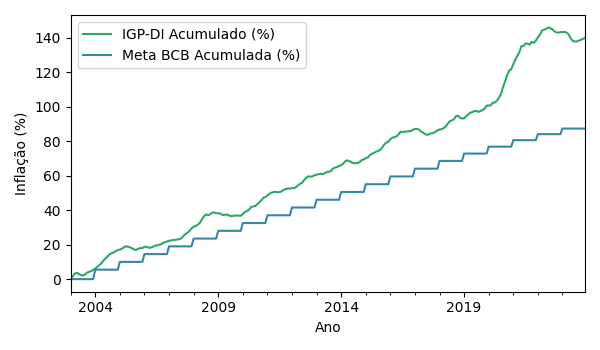
\includegraphics[]{fig/igpdi_96_24_t.png}\\
	\footnotesize{\textbf{Fonte}: o próprio autor, dados fornecidos pelo Banco Central e Fundação Getúlio Vargas.}
	\label{fig:igpdiacum}
\end{figure}

Na seção subsequente, observar-se-á que as principais fontes de inflação histórica no Brasil são associadas a políticas desenvolvimentistas e expansionistas, cuja contrapartida no crescimento da produção real da economia foi inferior ao necessário para evitar descompasso na elevação da base monetária. Nota-se que a inflação estrutural e a inflação inercial se sobressaltaram na economia brasileira, principalmente nas décadas de 1980 e 1990, até a execução bem-sucedida do Plano Real.


\chapter{Elementos Sobre Economia Brasileira}

Nessa seção, inicia-se a contextualização da história econômica do Brasil, assim como a análise do comportamento da política monetária ao longo do tempo. É feito, também, um detalhamento das principais características das políticas econômicas conduzidas por cada governo de 2003 a 2023 e seus impactos sobre o cenário econômico nacional.

\section{Governos do Século XX}

% TODO: O cenário econômico brasileiro entre a década de 80 e 90 foi marcado por anos de inflação recorrente, o regime militar deixara uma dívida externa estratosférica para os governos seguintes que tinham como principal meta o controle dos preços por meio de planos de estabilização. Sabe-se que todos os planos fracassaram na tentativa de conter o avanço da inflação, como explicam Moran e Witte (1993, p. 120): “No Brasil, são notórias as tentativas de conter este processo, a maioria não obteve o sucesso desejado por vários motivos. [...] dentre os quais destacam o Plano Cruzado I, o Plano Cruzado II, o Plano Bresser, o Plano Verão, o Plano Collor I e o Plano Collor II.”.

A bagagem econômica herdada dos diversos governos do século XX no Brasil teve um impacto duradouro na economia e na capacidade do país de implementar políticas macroeconômicas eficazes. Durante as décadas de 1950 e 1960, os governos de Getúlio Vargas e Juscelino Kubitschek adotaram políticas desenvolvimentistas que promoveram a industrialização acelerada e a expansão da infraestrutura, muitas vezes financiadas por meio de déficit público \cite{bielschowsky_2022_a}. Essas políticas resultaram em um crescimento econômico robusto, mas também em um aumento significativo da dívida pública e das pressões inflacionárias.

Sob o governo de Getúlio Vargas, a criação da Petrobras e da Companhia Siderúrgica Nacional (CSN) marcou um período de forte intervenção estatal na economia. O Estado Novo de Vargas (1937-1945) e seu segundo governo (1951-1954) buscaram consolidar a indústria de base no Brasil, visando reduzir a dependência de importações e fortalecer o mercado interno. Embora essas iniciativas tenham contribuído para a modernização da economia brasileira, elas também levaram a um aumento dos gastos públicos e ao crescimento da dívida externa \cite{fabiogiambiagi_2016_economia}.

Durante o governo de Juscelino Kubitschek (1956-1961), a política econômica se concentrou no Plano de Metas, que buscava ``50 anos em 5'' de desenvolvimento. Esse plano incluiu a construção de Brasília, a nova capital federal, e a expansão da infraestrutura de transporte e energia. Embora esses projetos tenham impulsionado a industrialização e o crescimento econômico, eles também resultaram em um aumento significativo do déficit público e da inflação \cite{bielschowsky_2022_a}. A rápida expansão foi financiada por meio de empréstimos externos, deixando o país vulnerável a crises de balanço de pagamentos.

Nos anos de 1960, a instabilidade política e econômica levou ao golpe militar de 1964, que instaurou um regime autoritário com uma nova agenda econômica. O governo militar inicialmente adotou medidas de austeridade para controlar a inflação e estabilizar a economia. Contudo, o período mais notável de crescimento, conhecido como o "milagre econômico brasileiro" (1968-1973), foi caracterizado por investimentos massivos em infraestrutura e pela abertura econômica. Esse crescimento foi impulsionado por políticas fiscais e monetárias expansivas, que, embora tenham gerado um aumento substancial do produto interno bruto (PIB), também ampliaram a dívida externa e interna \cite{amaurypatrickgremaud_2009_economia}.

O ``milagre econômico'' foi marcado por grandes projetos, como a construção da Rodovia Transamazônica e a usina de Itaipu, que demandaram enormes recursos financeiros. Embora esses projetos tenham impulsionado a economia, eles também aumentaram as pressões inflacionárias. Além disso, a concentração de renda e a repressão aos movimentos sociais geraram tensões sociais significativas. O choque do petróleo de 1973 exacerbou as vulnerabilidades econômicas, pois aumentou os custos de importação de energia e pressionou ainda mais a balança de pagamentos.

Isso fez com que a década de 1980, chamada de ``década perdida'', fosse marcada por estagnação econômica, hiperinflação e crise da dívida externa. A política econômica dos governos militares posteriores, particularmente sob a presidência de João Figueiredo (1979-1985), foi incapaz de lidar com as consequências dos choques externos e das políticas expansionistas anteriores. A moratória da dívida em 1987 simbolizou a profundidade da crise econômica \cite{fabiogiambiagi_2016_economia} na época. As tentativas de estabilização, como o Plano Cruzado (1986) durante o governo de José Sarney, falharam em resolver os problemas estruturais e levaram a surtos de hiperinflação.

O Plano Cruzado tentou controlar a inflação por meio do congelamento de preços e salários e da introdução de uma nova moeda, o cruzado. Inicialmente, o plano teve sucesso em reduzir a inflação, mas a falta de controle sobre os gastos públicos e a resistência política levaram ao seu fracasso. A inflação retornou, exacerbada pela falta de ajustes estruturais e pela deterioração das contas públicas \cite{fabiogiambiagi_1999_a}.

A transição para a democracia em 1985 trouxe novos desafios econômicos. O governo de Fernando Collor (1990-1992) implementou o Plano Collor, que incluía o confisco de depósitos bancários e a tentativa de liberalização econômica. Embora tenha reduzido temporariamente a inflação, o plano causou uma grave recessão econômica e enfrentou forte oposição política, resultando em sua rápida deterioração e na posterior hiperinflação \cite{lacerda_2010_economia}.

Durante o governo de Itamar Franco (1992-1995), o Brasil finalmente começou a estabilizar sua economia com o Plano Real, liderado pelo então Ministro da Fazenda Fernando Henrique Cardoso. O plano introduziu uma nova moeda, o real, e implementou âncoras cambiais e políticas fiscais rígidas. Essas medidas conseguiram estabilizar a inflação e criar uma base para o crescimento econômico sustentável. O sucesso do Plano Real foi um ponto de inflexão na história econômica do Brasil, marcando o fim de um ciclo de políticas populistas e instabilidade econômica \cite{lacerda_2010_economia}.

A instabilidade econômica e a subsequente estabilização pela qual o Brasil passou no período anterior e posterior ao Plano Real é claramente observada nas variações do Índice Geral de Preços - Disponibilidade Interna (IGP-DI). A Figura \ref{fig:igpdi}, a seguir, apresenta a série temporal do comportamento da inflação entre 1985 e 1996 no Brasil, com destaque para as diversas tentativas de estabilização realizadas.

\begin{figure}[H]
	
	\caption{Comportamento da Inflação Mensal - IGP-DI - 1985-1996 (\%)}
	
	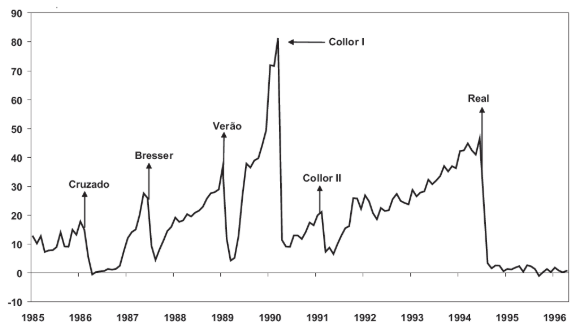
\includegraphics[]{fig/igp-di.png}\\
	
	\footnotesize Fonte: FGV.
	
	\label{fig:igpdi}
	
\end{figure}

Com destaque, a inflação no Brasil (Figura \ref{fig:igpdi}), observou diversos choques resultantes de políticas ineficazes no controle dos preços. O legado deixado pelo governos populistas do século XX, com suas políticas desenvolvimentistas e intervenções estatais, foi uma economia caracterizada por altas taxas de inflação, dívida pública crescente e instabilidade macroeconômica. A implementação do RMI em 1999 representou um esforço para romper com esse passado e adotar uma política monetária mais disciplinada e previsível, visando garantir a estabilidade de preços e promover o crescimento sustentável a longo prazo \cite{amaurypatrickgremaud_2009_economia}.

\section{Transição para a Estabilidade: Plano Real e a Introdução do RMI}

O Plano Real, implementado em 1994 durante o governo de Itamar Franco e sob a liderança do então Ministro da Fazenda Fernando Henrique Cardoso, marcou um ponto de inflexão na luta contra a inflação no Brasil. O plano envolveu uma série de medidas macroeconômicas, incluindo a criação de uma nova moeda, o real, a introdução de âncoras cambiais e a implementação de políticas fiscais rigorosas \cite{amaurypatrickgremaud_2009_economia}. Essas medidas conseguiram estabilizar a inflação e restaurar a confiança na economia brasileira.

A estabilidade alcançada pelo Plano Real criou as condições necessárias para a adoção do Regime de Metas de Inflação (RMI) em 1999. Esse novo regime, que enfatiza a transparência e a credibilidade das políticas monetárias, representou uma mudança de paradigma na abordagem do Brasil ao controle da inflação. Ao focar em metas de inflação como guia principal para a política monetária, o Banco Central do Brasil conseguiu ancorar as expectativas inflacionárias e promover um ambiente macroeconômico mais estável.

A implementação do Plano Real começou com uma série de medidas preparatórias, conhecidas como o Programa de Ação Imediata (PAI), que visavam reduzir a inércia inflacionária e estabilizar a economia antes da introdução da nova moeda. Essas medidas incluíram o ajuste fiscal, a redução do déficit público e a liberalização do comércio. Em julho de 1994, o real foi finalmente introduzido, substituindo o cruzeiro real a uma taxa de paridade inicial de 1:1 com o dólar norte-americano. A âncora cambial foi uma ferramenta crucial para estabilizar as expectativas inflacionárias e fortalecer a credibilidade da nova moeda \cite{silva_2002_plano}. 

A introdução do real foi acompanhada por uma política monetária restritiva, com altas taxas de juros para controlar a demanda agregada e evitar pressões inflacionárias. O governo também adotou um regime de câmbio fixo, permitindo que o Banco Central interviesse para manter a paridade da moeda. Essas medidas foram fundamentais para o sucesso inicial do Plano Real, que conseguiu reduzir a inflação anual de mais de 2.000\% em 1993 para menos de 10\% em 1996 \cite{fabiogiambiagi_1999_a}.

O sucesso do Plano Real não foi isento de desafios. A âncora cambial, enquanto eficaz no curto prazo, gerou pressões sobre a balança de pagamentos do Brasil, levando a um aumento do déficit em conta corrente. Além disso, a apreciação do real tornou as exportações brasileiras menos competitivas, aumentando a dependência de capital externo para financiar o déficit. Esses desequilíbrios se tornaram evidentes durante as crises financeiras internacionais da segunda metade da década de 1990, como a crise do México (1994-1995), a crise asiática (1997) e a crise da Rússia (1998) \cite{santna_2002_crises}.

Em resposta a essas crises e às pressões cambiais crescentes, o governo brasileiro decidiu abandonar a âncora cambial em janeiro de 1999 e adotar um regime de câmbio flutuante. Essa mudança foi acompanhada pela introdução do Regime de Metas de Inflação (RMI), que visava ancorar as expectativas inflacionárias por meio da transparência e previsibilidade das ações do Banco Central. Sob o RMI, o Conselho Monetário Nacional estabelece metas de inflação anuais, e o Banco Central utiliza as operações de \textit{open market}, redesconto e depósito compulsório como  principais instrumentos para atingir essas metas.

% TODO: No segundo mandato de FHC, entre 1999 e 2002, o país precisou recorrer ao Fundo Monetário Internacional (FMI) para enfrentar o problema externo, recebendo acote de ajuda em torno de U$ 40 bilhões. O acordo com o FMI enfrentou duas adversidades, Giambiagi et al. (2011) explicam que a desconfiança referente a não desvalorização do câmbio por parte do mercado e o desprezo pelo Congresso com relação a medida de contribuição previdenciária, imposta pelo plano, levou a rejeição da medida pelos congressistas e aumentou o pessimismo, acelerando o processo de perda de divisas.

A transição para o RMI representou uma mudança significativa na política monetária do Brasil. Ao invés de se concentrar exclusivamente no controle do câmbio, o Banco Central passou a focar na estabilidade de preços como seu principal objetivo. Essa abordagem permitiu uma maior flexibilidade na condução da política monetária, facilitando a resposta a choques econômicos internos e externos. A transparência do regime de metas também aumentou a credibilidade das políticas do Banco Central, ajudando a ancorar as expectativas inflacionárias e a reduzir a inflação de forma sustentável.

Nos primeiros anos do RMI, a economia brasileira enfrentou desafios significativos, incluindo uma crise cambial em 1999 e um cenário internacional adverso. No entanto, a política monetária firme e a disciplina fiscal contribuíram para a estabilização da economia. A inflação, que chegou a 8,9\% em 1999, foi gradualmente reduzida, atingindo 5,97\% em 2002. A credibilidade do Banco Central e a eficácia do RMI foram reforçadas pela consistência das políticas adotadas, mesmo diante de adversidades \cite{fabiogiambiagi_1999_a}.

Os governos de Fernando Henrique Cardoso (1995-2002) implementaram reformas estruturais importantes que complementaram a estabilidade macroeconômica promovida pelo Plano Real e pelo RMI. Entre essas reformas estavam a privatização de empresas estatais, a liberalização do mercado financeiro e a promoção de ajustes fiscais. Essas medidas contribuíram para aumentar a eficiência econômica e trazer ao Brasil características mais semelhantes às de países desenvolvidos \cite{fabiogiambiagi_2016_economia}.

No início dos anos 2000, o Brasil começou a colher os frutos das reformas e da estabilidade macroeconômica. A economia cresceu, a inflação permaneceu sob controle e a dívida pública passou a ser mais controlada. Apesar de parte do crescimento ter sido eclipsado pela crise energética de 2001 \cite{fabiogiambiagi_2016_economia}, as reformas monetárias foram um sucesso.

Em resumo, a transição para a estabilidade econômica no Brasil foi marcada pela implementação bem-sucedida do Plano Real e a adoção do Regime de Metas de Inflação. Essas mudanças representaram um rompimento com o passado de instabilidade e políticas populistas, estabelecendo as bases para um crescimento econômico sustentável e uma maior credibilidade das instituições econômicas brasileiras. A disciplina fiscal, a independência do Banco Central e a transparência das políticas monetárias foram elementos-chave para o sucesso dessa transição, que continua a influenciar positivamente a economia brasileira até os dias de hoje.

A partir de 2003, a economia brasileira passou por diversas mudanças econômicas e políticas que influenciaram a condução e os resultados do RMI. Os períodos analisados a seguir foram marcados por diferentes administrações que implementaram políticas econômicas distintas, refletindo na dinâmica inflacionária e na eficácia do regime. A seguir, é detalhada a evolução do quadro econômico brasileiro ao longo das diversas gestões.

\section{Período Lula (2003-2010)}

Durante o governo de Luiz Inácio Lula da Silva (2003-2010), o Brasil experimentou um período de forte crescimento econômico, impulsionado pela alta nos preços das \textit{commodities} e um aumento significativo nos investimentos estrangeiros diretos. A gestão do Banco Central, sob a liderança de Henrique Meirelles, manteve uma política monetária rigorosa para controlar a inflação. A taxa SELIC foi usada de forma ativa para garantir que a inflação permanecesse dentro das metas estabelecidas pelo Conselho Monetário Nacional (CMN). Segundo \citeonline{silva_2016_politica}, a política fiscal contracionista adotada nos primeiros anos do governo Lula contribuiu para a credibilidade dos mandatos, permitindo uma redução gradual da taxa de juros sem comprometer a estabilidade dos preços.

O período também foi marcado por um aumento na credibilidade internacional do Brasil, com a economia apresentando crescimento robusto e uma significativa redução na vulnerabilidade externa. O superávit primário foi mantido, garantindo um controle mais rígido das contas públicas e contribuindo para a estabilidade macroeconômica. A combinação de uma política fiscal responsável com uma política monetária eficiente permitiu que o Brasil navegasse com sucesso por um cenário econômico global inicialmente favorável, mas que se tornou desafiador com a crise financeira de 2008 \cite{fabiogiambiagi_2016_economia}.

A crise financeira global de 2008 representou um grande desafio para a economia brasileira. O governo Lula, em resposta, adotou uma série de medidas para mitigar os impactos da crise, incluindo a redução da taxa SELIC e a implementação de pacotes de estímulo fiscal para sustentar o consumo e o investimento. Essas medidas, associadas à robustez do sistema financeiro brasileiro e à atuação prudente do Banco Central, permitiram que o Brasil enfrentasse a crise de maneira mais resiliente em comparação com muitas outras economias emergentes e desenvolvidas.

Além das políticas de estabilização econômica, o governo Lula implementou programas sociais de grande alcance, como o Bolsa Família, que contribuíram para a redução da pobreza e da desigualdade social. Esses programas tiveram um efeito positivo no aumento da demanda interna, apoiando o crescimento econômico. A inclusão social promovida por esses programas não apenas melhorou as condições de vida de milhões de brasileiros, mas também criou um mercado consumidor interno mais dinâmico, o que foi fundamental para o crescimento sustentado da economia durante esse período.

No entanto, o aumento do consumo e a expansão dos programas sociais também colocaram pressão sobre a inflação. A execução do RMI levantou críticas sobre os altos custos dos empréstimos e o impacto negativo sobre o investimento e o crescimento econômico a longo prazo. Dessa forma, o regime de metas de inflação trouxe impactos para a economia brasileira durante o governo Lula, proporcionando estabilidade de preços, mas também impondo restrições à flexibilidade econômica.

TODO: passar citações para refs.bib

\section{Período Dilma Rousseff (2011-2016)}
O governo de Dilma Rousseff (2011-2016) enfrentou desafios econômicos significativos, incluindo uma desaceleração econômica e aumento das pressões inflacionárias. A política econômica adotada durante este período foi caracterizada por uma expansão fiscal e intervenções frequentes nos preços administrados, como combustíveis e energia, o que dificultou o controle da inflação. A credibilidade do governo foi colocada em questão devido ao uso de medidas não convencionais e à percepção de interferência política no Banco Central. Como resultado, a inflação frequentemente excedeu as metas estabelecidas, exigindo aumentos abruptos na taxa de juros para tentar trazer a inflação de volta ao intervalo meta \cite{carvalho_2016_growth}.

A implementação de políticas expansionistas, conhecidas como "nova matriz econômica", buscava incentivar o crescimento econômico através do aumento dos gastos públicos e subsídios a setores estratégicos. No entanto, essas políticas resultaram em um aumento do déficit fiscal e da dívida pública, o que elevou as expectativas inflacionárias. As desonerações tributárias e a política de controle de preços contribuíram para a deterioração das contas públicas e limitaram a capacidade do Banco Central de utilizar a política monetária para controlar a inflação de maneira eficaz.

O contexto internacional também influenciou significativamente a economia brasileira durante o governo Dilma. A queda nos preços das \textit{commodities} e a desaceleração do crescimento global impactaram negativamente a balança comercial brasileira, reduzindo as receitas de exportação e aumentando a vulnerabilidade externa do país. Esses fatores externos, aliados às políticas domésticas expansionistas, intensificaram as pressões inflacionárias e tornaram o ambiente econômico mais desafiador para a manutenção da estabilidade dos preços.

A falta de coordenação entre as políticas fiscal e monetária foi um dos principais problemas enfrentados durante esse período. Enquanto o Banco Central tentava controlar a inflação através do aumento da taxa SELIC, a política fiscal expansionista do governo gerava pressões contrárias, dificultando o alcance das metas inflacionárias. Esse descompasso entre as políticas minou a eficácia do RMI e aumentou a incerteza econômica, afetando negativamente a confiança dos investidores e consumidores.

Ao final do segundo mandato de Dilma Rousseff, a economia brasileira enfrentava uma grave recessão, com inflação elevada e desemprego em alta. A crise política e econômica culminou no \textit{impeachment} da presidente em 2016. A gestão subsequente herdou um cenário econômico complexo, marcado pela necessidade urgente de ajustes fiscais e de recuperação da credibilidade. Esse período evidenciou a importância de uma coordenação eficaz entre as políticas fiscal e monetária para a manutenção da estabilidade econômica e do controle inflacionário.

\section{Período Michel Temer (2016-2018)}

Com a chegada de Michel Temer à presidência em 2016, houve uma mudança significativa na política econômica do Brasil. Após o \textit{impeachment} de Dilma Rousseff, o governo Temer buscou implementar uma série de reformas estruturais com o objetivo de restaurar a confiança dos mercados e estabilizar a economia brasileira. Entre as principais medidas adotadas estavam a reforma trabalhista e a  proposta de emenda à constituição (PEC) do teto dos gastos, que limitou o crescimento dos gastos públicos à taxa de inflação do ano anterior por vinte anos. Essas reformas foram vistas como cruciais para o ajuste fiscal e para a recuperação da credibilidade econômica do país.

A gestão do Banco Central sob a liderança de Ilan Goldfajn foi marcada por um compromisso firme com o controle da inflação e a estabilização macroeconômica. Uma das primeiras ações de Goldfajn foi ancorar as expectativas inflacionárias, o que permitiu uma redução gradual e consistente da taxa SELIC ao longo de seu mandato. Essa abordagem contribuiu significativamente para a redução da inflação, que voltou a se situar dentro das metas estabelecidas pelo Conselho Monetário Nacional (CMN) após os elevados índices registrados no final do governo Dilma Rousseff.

Além das reformas estruturais e da política monetária rigorosa, o governo Temer também enfrentou o desafio de recuperar a confiança dos investidores e reverter a recessão econômica. O impacto positivo dessas medidas começou a ser percebido já em 2017, quando o Brasil registrou um leve crescimento econômico após dois anos de recessão profunda. A combinação de um ambiente regulatório mais favorável e de uma política monetária estável ajudou a atrair investimentos e a estimular a recuperação do emprego e da renda.

No entanto, o governo Temer também enfrentou dificuldades, incluindo a resistência política às reformas e os escândalos de corrupção que marcaram seu mandato. Apesar das controvérsias, a continuidade da política econômica voltada para a austeridade fiscal e a estabilidade monetária foi fundamental para consolidar os avanços obtidos na estabilização da economia.

\section{Período Jair Bolsonaro (2019-2022)}

O governo de Jair Bolsonaro (2019-2022) enfrentou desafios econômicos significativos, incluindo a pandemia de COVID-19, que impactou profundamente a economia global e doméstica. A resposta inicial do governo incluiu medidas fiscais expansivas para mitigar os efeitos econômicos da pandemia, como o auxílio emergencial e programas de manutenção de emprego, o que aumentou as preocupações inflacionárias. Essas medidas, apesar de essenciais para a proteção social e a manutenção da renda, pressionaram as contas públicas e elevaram a relação dívida/PIB do país.

Durante esse período, Roberto Campos Neto, presidente do Banco Central, manteve uma postura vigilante, ajustando a taxa SELIC conforme necessário para conter as pressões inflacionárias. Inicialmente, a taxa de juros foi reduzida para níveis historicamente baixos a fim de estimular a economia (2\%), mas a partir de 2021, devido ao aumento das pressões inflacionárias, houve um ciclo de elevação da SELIC para controlar a inflação, gerando uma alta significativa (13,75\%).

A pandemia também causou disrupções significativas nas cadeias de suprimentos globais, resultando em aumentos nos preços dos alimentos, energia e outros bens essenciais. Esses choques de oferta, combinados com uma depreciação cambial significativa, contribuíram para o aumento da inflação no Brasil. Apesar dessas dificuldades, o Banco Central adotou medidas de política monetária para evitar que a inflação se descontrolasse, influenciando proativamente a taxa de juros.

A política fiscal do governo Bolsonaro, particularmente durante a pandemia, foi caracterizada por um aumento substancial nos gastos públicos para enfrentar a crise sanitária e econômica. No entanto, essa expansão fiscal foi acompanhada de uma preocupação crescente com a sustentabilidade das contas públicas. A combinação de um elevado déficit fiscal e a crescente dívida pública gerou incertezas sobre a capacidade do governo de cumprir as metas fiscais e de manter a estabilidade econômica a longo prazo.

Além dos desafios econômicos, o governo Bolsonaro também enfrentou uma série de crises políticas que impactaram a economia. A relação tensa entre o poder executivo e os outros poderes, além das constantes mudanças nos ministérios, contribuiu para um ambiente de incerteza. No entanto, a independência formal do Banco Central, conquistada em 2021, foi vista como um passo importante para fortalecer o RMI e garantir uma política monetária mais eficiente e menos sujeita a pressões políticas, contribuindo para a estabilidade macroeconômica.

\section{Perspectivas Recentes e Desafios (2023)}

Atualmente, o Brasil enfrenta uma série de desafios e oportunidades econômicas. Um dos principais focos continua sendo o controle da inflação, que permanece sendo um ponto focal para o Banco Central. Sob a liderança de Roberto Campos Neto, a política monetária tem sido rigorosamente ajustada para garantir que a inflação fique dentro das metas estabelecidas, apesar das pressões inflacionárias globais e domésticas. Como é observado abaixo na Figura \ref{fig:ipcatgt}, o país tem enfrentado taxas de inflação frequentemente maiores do que o planejado e isso se acentuou de forma severa após 2020:

\begin{figure}[H]
	
	\caption{Variação do IPCA x Meta de Inflação (BCB) (\%)}
	
	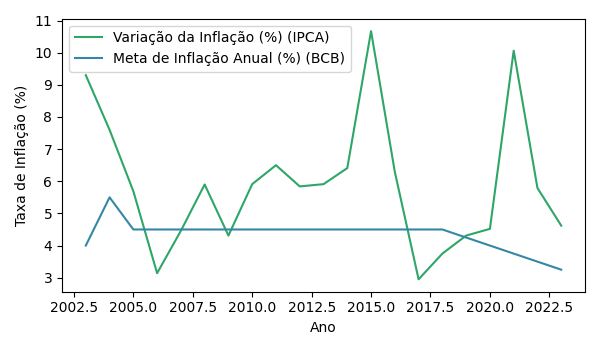
\includegraphics[]{fig/ibge_ipca_bcb_meta_99_23_t.png}\\
	
	\label{fig:ipcatgt}
	\footnotesize \textbf{Fonte}: o próprio autor, dados fornecidos pelo Banco Central e IBGE.
	
\end{figure}

É interessante notar como crises econômicas	globais tiveram impacto sobre o ritmo do crescimento da inflação no Brasil. Tanto em 2009, na crise do \textit{subprime}, quanto em 2019, com a crise do COVID-19, observou-se (Tabela \ref{fig:ipcatgt}) a incapacidade das metas de inflação acompanharem a expansão monetária realizada nos períodos de gerenciamento das crises, evidenciando a dificuldade em manter a inflação sob controle. Diante dessa complexidade, a próxima seção traz a escolha de modelos econométricos que propõem formas de analisar o comportamento da política monetária diante de tais cenários econômicos.

% \section{}

% A alta taxa de juros necessária para manter a inflação sob controle tem um impacto negativo sobre o crescimento econômico e o emprego. Os custos de empréstimos elevados desincentivam investimentos e consumo, limitando o crescimento do PIB

% A pressão para atingir metas anuais pode levar a uma política monetária excessivamente restritiva ou expansiva, prejudicando a estabilidade econômica de longo prazo. A tentativa de atingir metas de curto prazo pode negligenciar problemas estruturais mais profundos na economia brasileira

% Dominancia fiscal?

\chapter{Metodologia}

Há diversos modelos econométricos capazes de analisar a relação entre a política monetária e a inflação. Para o estudo, foi selecionado o modelo de vetores autorregressivos (VAR), que é amplamente utilizado para compreender a relação dinâmica entre múltiplas séries temporais, compostas por variáveis de política monetária como taxa de juros, índices de inflação e variáveis macroeconômicas, como PIB e taxa de câmbio. 

O modelo VAR será utilizado porque permite analisar a interação entre múltiplas variáveis econômicas de forma dinâmica, sem impor restrições \textit{a priori} sobre a causalidade entre elas. Em um contexto como o da inflação no Brasil, onde diversas variáveis interagem de maneira complexa, o VAR se destaca por sua capacidade de modelar essas inter-relações de forma simultânea. Diferentemente de modelos estruturais, o VAR trata todas as variáveis como endógenas, o que é crucial para capturar adequadamente a resposta da política monetária e outras variáveis econômicas a choques inesperados, como os de oferta e demanda.

Como o objetivo deste estudo é analisar tanto a dinâmica inflacionária de oferta quanto de demanda, o VAR oferece a flexibilidade necessária para modelar essas influências e testar como a política monetária deve ser ajustada para alcançar os objetivos propostos pelo regime de metas de inflação. Em sua extensão, o modelo VAR oferece funções de resposta a impulsos (IRF) e decomposição de variância (VD), que são utilizados para estudar o impacto de um choque na inflação sobre a política monetária ao longo do tempo.

\section{Modelo}

Para a construção do modelo VAR, o primeiro passo é garantir que as variáveis utilizadas no modelo sejam estacionárias. A estacionariedade é fundamental para evitar resultados espúrios, ou seja, resultados que indicam uma relação de longo prazo inexistente entre as variáveis. De acordo com Gujarati e Porter (2011), uma série temporal estacionária é aquela cujas propriedades estatísticas, como média, variância e autocorrelação, não mudam ao longo do tempo. A verificação da estacionariedade é realizada por meio de testes como o Dickey-Fuller aumentado (ADF) e o Phillips-Perron (PP), que testam a presença de raiz unitária na série temporal. Caso as séries não sejam estacionárias, é possível realizar diferenciações para atingir a estacionariedade \cite{gujarati_porter_2011}, como observado a seguir.

\subsection{Diferenciação de Séries Temporais}

A diferenciação de uma série temporal é um procedimento utilizado para tornar uma série não estacionária em estacionária, eliminando tendências e ciclos de longo prazo. A diferenciação consiste em calcular a diferença entre os valores consecutivos de uma série. Para uma observação de uma série temporal \( y_t \), a primeira diferença é dada por:

\begin{equation}
	\Delta y_t = y_t - y_{t-1}
\end{equation}

onde:

\begin{itemize}
	\item \( y_t \) é o valor da série no período \( t \),
	\item \( y_{t-1} \) é o valor da série no período \( t-1 \),
	\item \( \Delta y_t \) é a primeira diferença da observação na série temporal.
\end{itemize}

A diferenciação de ordem \( d \), observada na equação \ref{eqn:diffsimple} a seguir, generaliza esse conceito. Quando a série precisa ser diferenciada mais de uma vez para se tornar estacionária, o processo pode ser repetido. De forma geral, a diferenciação de ordem \( d \) de uma observação \( y_t \) em uma série é definida como:

\begin{equation}
	\label{eqn:diffsimple}
	\Delta^d y_t = \Delta^{d-1}(y_t - y_{t-1})
\end{equation}

Para determinar corretamente como proceder com a diferenciação de uma série, surge a necessidade de verificar o número ideal de defasagens a ser utilizado no modelo. Nesse contexto, as seções subsequentes oferecem critérios que equilibram a complexidade do modelo e seu ajuste aos dados, auxiliando na escolha do número de defasagens apropriado ao penalizar a inclusão de parâmetros desnecessários, garantindo que o modelo não seja superajustado.

\subsection{Critério de Informação de Akaike (AIC)}

O Critério de Informação de Akaike (AIC) é um dos métodos mais amplamente utilizados para determinar o número ótimo de defasagens em modelos de séries temporais. Desenvolvido por Hirotugu Akaike, sua fórmula é dada por:

\begin{equation}
	AIC = -2 \ln(L) + 2k
\end{equation}

onde:

\begin{itemize}
	\item \( L \) é o valor da função de verossimilhança estimada para o modelo,
	\item \( k \) é o número de parâmetros estimados no modelo, incluindo as defasagens e o termo constante.
\end{itemize}

O AIC é construído de modo a favorecer modelos que maximizam a verossimilhança enquanto penaliza o número de parâmetros. Geralmente, quanto maior o número de parâmetros, melhor o ajuste do modelo aos dados. No entanto, um aumento no número de parâmetros pode levar a um modelo superajustado \textit{overfitting}, onde o modelo capta não apenas o padrão subjacente nos dados, mas também o ruído. Assim, o termo de penalização \( 2k \) busca corrigir esse problema.

Ao comparar diferentes modelos com defasagens variáveis, o modelo que apresenta o menor valor de AIC é escolhido como o modelo ótimo. No entanto, o AIC tende a ser mais permissivo em relação ao número de defasagens, selecionando frequentemente um número maior de \textit{lags} em comparação com outros critérios, como o Critério de Informação de Schwarz (BIC) ou o Critério de Hannan-Quinn, vistos a seguir.

\subsection{Critério de Informação de Schwarz (BIC)}

O Critério de Informação de Schwarz (BIC), também conhecido como Critério de Informação Bayesiano, tem fórmula muito parecida com o AIC:

\begin{equation}
	BIC = -2 \ln(L) + k \ln(n)
\end{equation}

A diferença chave entre os critérios é que o termo de penalização no BIC, \( k \ln(n) \), aumenta com o número de observações, tornando-o mais rigoroso conforme a amostra cresce. Isso implica que, para grandes amostras, o BIC tende a selecionar modelos com menos parâmetros em comparação ao AIC. No entanto, devido à sua penalização mais severa, o BIC pode, às vezes, subestimar o número de defasagens necessário, principalmente em séries onde há muita autocorrelação residual.

\subsection{Critério de Hannan-Quinn (HQIC)}

Desenvolvido por Edward Hannan e Barry Quinn, o HQIC oferece um meio-termo entre o AIC e o BIC em termos de penalização pela inclusão de parâmetros adicionais. A fórmula do HQIC é:

\begin{equation}
	\label{eqn:hannanquinn}
	HQIC = -2 L_{max} + 2k \ln(\ln(n))
\end{equation}

onde:

\begin{itemize}
	\item \( L_{max} \) é o valor da função (\textit{log-likelihood}) de verossimilhança estimada para o modelo,
	\item \( k \) é o número de parâmetros estimados no modelo,
	\item \( n \) é o número de observações na série temporal.
\end{itemize}

Como é observado na Equação \ref{eqn:hannanquinn}, o HQIC penaliza a inclusão de parâmetros de maneira mais severa que o AIC, mas menos rigorosa que o BIC. O termo \( 2k \ln(\ln(n)) \) cresce mais lentamente do que o termo \( k \ln(n) \) no BIC, tornando o HQIC uma escolha apropriada em situações onde o BIC pode ser muito conservador e o AIC, muito permissivo.

O HQIC é particularmente útil em séries temporais de tamanho intermediário, onde o número de observações não é suficientemente grande para justificar o uso do BIC, mas onde ainda é necessário um controle maior sobre o número de defasagens em comparação com o AIC. 

Como os outros critérios, o HQIC não garante que o modelo selecionado seja o "verdadeiro" modelo subjacente, apenas que ele representa um bom compromisso entre complexidade e ajuste. Seu uso, assim como o AIC e o BIC, deve ser acompanhado de outras análises diagnósticas para garantir a adequação do modelo às características da série temporal.

Para proceder com a estimação do modelo, ainda resta verificar se as séries defasadas são efetivamente estacionárias após a diferenciação, sendo preciso realizar um teste formal de raiz unitária, como o teste de Dickey-Fuller Aumentado (ADF) ou o teste de Phillips-Perron (PP), descritos a seguir. 

\subsection{Teste de Dickey-Fuller Aumentado}

Extensão do teste de Dickey-Fuller original, o teste ADF adiciona termos de defasagem das diferenças da variável dependente ao modelo para capturar qualquer autocorrelação nos resíduos. Isso permite que o teste corrija problemas de autocorrelação, que podem invalidar os resultados do teste de Dickey-Fuller padrão em séries temporais complexas, como é comum em séries macroeconômicas e financeiras.  A equação geral do teste ADF pode ser representada da seguinte forma:

\begin{equation}
	\Delta y_t = \alpha + \beta t + \gamma y_{t-1} + \sum_{i=1}^{p} \delta_i \Delta y_{t-i} + \epsilon_t
\end{equation}

onde:

\begin{itemize}
	\item \( \Delta y_t \) é a primeira diferença da série temporal \( y_t \),
	\item \( \alpha \) é o intercepto ou termo constante,
	\item \( \beta \) é o coeficiente da tendência temporal \( t \),
	\item \( \gamma \) é o coeficiente de \( y_{t-1} \), utilizado para testar a presença de raiz unitária (com a hipótese nula \( H_0: \gamma = 0 \)),
	\item \( \delta_i \) são os coeficientes das defasagens \( \Delta y_{t-i} \), introduzidos para ajustar a autocorrelação,
	\item \( \epsilon_t \) são os resíduos da equação.
\end{itemize}

A inclusão das defasagens \( \Delta y_{t-i} \) permite ao teste ADF lidar com séries temporais que apresentam autocorrelação serial nos erros. O número de defasagens \( p \) é selecionado com base em critérios de informação, como o Critério de Informação de Akaike (AIC) ou o Critério de Informação Bayesiano (BIC), de modo a garantir que os erros \( \epsilon_t \) sejam não correlacionados e distribuídos de forma aproximadamente normal.

A hipótese nula do teste ADF é que a série possui uma raiz unitária (\( H_0: \gamma = 0 \)), ou seja, que a série é não estacionária. Quando o valor calculado da estatística \( t \) é menor do que o valor crítico correspondente, a hipótese nula é rejeitada, indicando que a série é estacionária. Caso contrário, a série é considerada não estacionária e, portanto, apresenta uma raiz unitária. O teste ADF, assim como o teste de Phillips-Perron, pode ser ajustado para incluir apenas um termo constante, um termo de tendência, ou ambos, dependendo da natureza da série temporal.

Uma vantagem do teste ADF em relação ao Dickey-Fuller simples é sua robustez a formas mais gerais de autocorrelação nos resíduos, o que o torna amplamente utilizado em análises econométricas. Contudo, sua eficácia ainda depende da seleção adequada do número de defasagens, pois incluir muitas defasagens pode reduzir a potência do teste, enquanto incluir poucas pode deixar a autocorrelação nos resíduos não ajustada, comprometendo os resultados do teste.

\subsection{Teste de Phillips-Perron}

Visto que o ADF assume que os erros do modelo são homocedásticos, sendo uma potencial limitação em casos onde há heterocedasticidade ou autocorrelação nos resíduos, \citeonline{phillips_perron_1988} propuseram uma alternativa mais robusta, que é o teste de Phillips-Perron (PP). O teste é procedido sem a necessidade de incluir defasagens adicionais das diferenças como no ADF. A metodologia de Phillips-Perron se baseia na mesma equação \ref{eqn:adf_reg} de regressão do teste de Dickey-Fuller, que pode ser representada como:

\begin{equation}
	\label{eqn:adf_reg}
	\Delta y_t = \alpha + \beta t + \gamma y_{t-1} + \epsilon_t
\end{equation}

onde:

\begin{itemize}
	\item \( \Delta y_t \) é a diferença da série temporal \( y_t \),
	\item \( \alpha \) é o termo constante (ou intercepto),
	\item \( \beta \) é o coeficiente da tendência determinística \( t \),
	\item \( \gamma \) é o parâmetro que testa a raiz unitária, sendo \( H_0: \gamma = 0 \) o indicativo de presença de raiz unitária,
	\item \( \epsilon_t \) são os erros do modelo.
\end{itemize}

Diferentemente do ADF, o teste de Phillips-Perron utiliza uma correção não paramétrica para lidar com autocorrelação e heterocedasticidade nos erros \( \epsilon_t \). Em vez de adicionar defasagens para ajustar a autocorrelação serial, o teste PP ajusta a estatística \( t \) da regressão por meio de uma estimativa robusta da variância assintótica dos resíduos. Isso é feito através da seguinte modificação na estatística \( t \):

\begin{equation}
	Z_\alpha = \frac{\hat{\gamma}}{\widehat{\sigma}_{\gamma}}
\end{equation}

onde \( \hat{\gamma} \) é o coeficiente estimado da regressão e \( \widehat{\sigma}_{\gamma} \) é a estimativa robusta da variância assintótica de \( \hat{\gamma} \), que corrige para heterocedasticidade e autocorrelação dos erros \( \epsilon_t \).

\citeonline{phillips_perron_1988} mostram que o teste PP é assintoticamente equivalente ao ADF, mas com a vantagem de ser mais robusto a formas de heterocedasticidade que são comuns em séries temporais econômicas. De acordo com \citeonline{greene_2008_econometric_analysis}, o teste de Phillips-Perron é uma alternativa poderosa quando se deseja manter a simplicidade do modelo sem incluir muitas defasagens, sendo especialmente útil em amostras menores, onde a inclusão de muitas defasagens poderia reduzir a potência do teste.

Outro ponto importante é que o teste de Phillips-Perron, assim como o ADF, pode ser realizado sob diferentes hipóteses. Ele pode ser ajustado para incluir um termo constante, uma tendência determinística, ou ambos, dependendo das características da série temporal que se está analisando. Assim, ele oferece a flexibilidade necessária para lidar com uma ampla gama de séries temporais, desde aquelas com tendência até as que são puramente estacionárias.

De maneira semelhante ao teste ADF, os valores críticos do teste de Phillips-Perron são obtidos de tabelas específicas que levam em consideração a estrutura assintótica da série. O valor de \( \gamma \) deve ser comparado com os valores críticos apropriados, e a hipótese nula de raiz unitária (\( H_0: \gamma = 0 \)) é rejeitada se a estatística de teste for menor que o valor crítico, indicando que a série é estacionária.


Baseado na metodologia exposta, são coletados e tratados os dados pertinentes ao estudo. A seção seguinte descreve a origem e a função dos dados no momento da composição do modelo.

\section{Dados}

% variaveis do modelo, OK
% tsset,
% dfuller, pperron,          p < 0.05 = estacionario
% dfuller diff, pperron diff p < 0.05 = estacionario
% var v1 v2, lags(1/2)
% varsoc
% varstable
% predict err, resid
% summarize err
% tsline err, yline(COPY OF MEAN FROM LAST CMD)
% varlmar (lagrange autocorr)
% granger test to check causality (p < 0.05 -> v1 predicts v2)

% https://www3.bcb.gov.br/sgspub/localizarseries/localizarSeries.do?method=prepararTelaLocalizarSeries


% IPCA = https://www.ibge.gov.br/estatisticas/economicas/precos-e-custos/9256-indice-nacional-de-precos-ao-consumidor-amplo.html?=&t=series-historicas
% IPA-EP-DI = https://extra-ibre.fgv.br/IBRE/sitefgvdados/visualizaconsulta.aspx
% SELIC = https://www.gov.br/receitafederal/pt-br/assuntos/orientacao-tributaria/pagamentos-e-parcelamentos/taxa-de-juros-selic#Taxa_de_Juros_Selic
% PIB = http://www.ipeadata.gov.br/ExibeSerie.aspx?serid=521274780&module=M
% CAMBIO = http://www.ipeadata.gov.br/ExibeSerie.aspx?stub=1&serid=38590&module=M


O Banco Central é a principal fonte de informações para indicadores monetários e de inflação, disponibilizando séries temporais detalhadas sobre a taxa SELIC, as metas anuais de inflação e outras variáveis relevantes sob o contexto da política monetária. Esses dados são utilizados na composição do modelo econométrico através da seleção das séries de metas anuais de inflação e das taxas mensais de juros SELIC. 

Além dos dados do Banco Central, o Instituto Brasileiro de Geografia e Estatística (IBGE) forneceu dados mensais da evolução do IPCA, a Fundação Getúlio Vargas forneceu os dados de IGP-DI e IPA-EP-DI e o Instituto de Pesquisa Econômica Aplicada (IPEA) forneceu dados para compor as variáveis do PIB (a estimativa do IPEA feita via interpolação dos valores trimestrais divulgados pelo IBGE nos permite fácil conciliação com as outras bases de dados) e da taxa de câmbio. O IBGE também disponibiliza o Índice de Preços ao Produtor, porém o IPA-EP-DI foi preferido dada o fato do estudo analisar o impacto da inflação desde 2003 e o IPP possuir dados históricos apenas a partir de 2011.

O IPA-EP-DI separa os preços em três categorias: bens finais, bens intermediários, e matérias-primas brutas. Isso permite uma análise mais granular dos impactos de oferta, já que muitos choques de oferta começam com o aumento dos preços das matérias-primas ou dos bens intermediários, que depois afetam os bens finais.
Com essa estrutura, é possível identificar com maior clareza em que ponto da cadeia produtiva os choques de oferta estão ocorrendo e como esses aumentos se propagam até os preços finais. A capacidade de separar os preços das matérias-primas de outros estágios oferece uma visão mais clara das dinâmicas da inflação de oferta.

O IPA-EP-DI é uma ferramenta mais adequada para medir a inflação de oferta do que outros índices da FGV como o Índice de Preços ao Produtor Amplo - Mercado (IPA-M), pois oferece uma segmentação detalhada dos preços ao longo da cadeia produtiva, permitindo identificar como os aumentos nos custos dos insumos básicos afetam os preços finais, sendo particularmente útil para análises sobre a origem e o impacto dos choques de oferta na economia.

O PIB foi deflacionado para o ano de 2003 utilizando o IGP-DI como deflator, isolando o efeito das flutuações de preços e garantindo que as comparações ao longo do período estudado reflitam mudanças reais na produção, e não apenas na inflação. O IGP-DI foi escolhido como o índice deflator por ser um indicador abrangente que capta a variação de preços em diferentes setores da economia, incluindo o atacado, o consumidor e a construção civil, tornando-o uma medida robusta para corrigir o PIB nominal e convertê-lo em termos reais.

A taxa de câmbio utilizada no estudo expressa o valor da moeda brasileira em relação ao dólar americano. As observações diárias foram transformadas em observações mensais através do cálculo de média simples. Isso foi feito para compatibilizar essa variável com as demais.

A meta de inflação, definida pelo Conselho Monetário Nacional (CMN) e conduzida pelo BCB, serve como um guia para as expectativas inflacionárias e para a condução das taxas de juros via taxa Selic. Ao incluir essa variável no modelo, é possível verificar se a inflação real (capturada pelo IPA-EP-DI no lado de oferta e pelo IPCA no lado de demanda) converge para a meta estabelecida, o que permite avaliar o sucesso ou as deficiências da política monetária no controle da inflação ao longo do tempo. Além disso, essa variável permite observar como a política monetária responde a diferentes tipos de choques inflacionários ao longo do período analisado.

Após descrever as variáveis das diferentes fontes de dados, é apresentada, a seguir, a Tabela \ref{table:vars}, que sintetiza as variáveis, suas origens e as siglas que foram adotadas durante a execução da rotina econométrica feita no \textit{software} STATA:

\vspace{0.2cm}
\begin{table}[H]
	\caption{Variáveis Utilizadas}
	\centering
	\rowcolors{2}{gray!8}{white}
	\begin{tabular}{ | l || c | l | }
		\hline
		\textbf{Variável}                                                  & \textbf{Origem} & \textbf{Sigla} \\
		\hline
		\textbf{Índice de Preços ao Consumidor Amplo (IPCA)}               & IBGE            & ipca           \\
		\textbf{Índice Geral de Preços - Disponibilidade Interna (IGP-DI)} & FGV             & igpdi          \\
		\textbf{Índice de Preços ao Produtor Amplo (IPA-EP-DI)}            & FGV             & d\_ipa\_ep\_di \\
		\textbf{Produto Interno Bruto Real}                                & Ipeadata        & d\_pibdefl2003 \\
		\textbf{Taxa de Juros SELIC}                                       & BCB             & selic          \\
		\textbf{Meta de Inflação}                                          & BCB             & metabcb        \\
		\textbf{Câmbio Real}                                               & BCB             & d\_rate        \\
		\hline
	\end{tabular}
	\vspace{1ex}
	\label{table:vars}
	
	\raggedright{
		\noindent \footnotesize{Fonte: o próprio autor.}}
\end{table}

\vspace{-0.2cm}
\vspace{0.5cm}

%%%%%%%%%%%%%%%%%%%%%%%%%%%%%%%%%%%%%%%%%%%%%%%%%%%%%%%%%%%%%%%%%%%

A seguir, definimos dois modelos VAR, sendo que um deles inclui o IPCA como variável \textit{proxy} da inflação de demanda e o outro inclui o IPA-EP-DI como \textit{proxy} da inflação de oferta, como observado nas equações \ref{eqn:varipca} e \ref{eqn:varipa}:

\begin{equation}
	\label{eqn:varipca}
	\text{ipca} = \alpha +  \beta_{1}\text{metabcb} + \beta_{2}\text{selic} + \beta_{3}\text{d\_pibdefl2003} + \beta_{4}\text{d\_rate} + u_{t}
\end{equation}
\begin{equation}
	\label{eqn:varipa}
	\text{d\_ipa\_ep\_di} = \alpha +  \beta_{1}\text{metabcb} + \beta_{2}\text{selic} + \beta_{3}\text{d\_pibdefl2003} + \beta_{4}\text{d\_rate} + u_{t}
\end{equation}
\vspace{0ex}

Para verificar a relação entre as variáveis, propõe-se o uso do teste de causalidade de Granger, visto em sequência.

\section{Teste de Causalidade de Granger}

O teste de causalidade de Granger, proposto por Clive Granger em 1969, é uma ferramenta fundamental para avaliar se uma variável \( X_t \) ajuda a prever outra variável \( Y_t \). O conceito de causalidade no sentido de Granger não se refere a uma causalidade no sentido tradicional, mas sim à ideia de que \( X_t \) é útil para prever \( Y_t \) além do que \( Y_t \) poderia prever com base apenas em suas próprias defasagens. Ou seja, se a inclusão das defasagens de \( X_t \) melhora a previsão de \( Y_t \), então \( X_t \) Granger-causa \( Y_t \).

Para testar a causalidade de Granger, consideram-se dois modelos de regressão linear autoregressiva para uma série temporal \( Y_t \):

\begin{equation}
	Y_t = \alpha_0 + \sum_{i=1}^{p} \alpha_i Y_{t-i} + \epsilon_t
\end{equation}

e

\begin{equation}
	Y_t = \beta_0 + \sum_{i=1}^{p} \beta_i Y_{t-i} + \sum_{i=1}^{p} \gamma_i X_{t-i} + \epsilon_t
\end{equation}

onde:

\begin{itemize}
	\item \( Y_t \) é a variável dependente,
	\item \( X_t \) é a variável candidata a Granger-causar \( Y_t \),
	\item \( \alpha_i \), \( \beta_i \), e \( \gamma_i \) são os coeficientes das defasagens das variáveis \( Y_t \) e \( X_t \),
	\item \( \epsilon_t \) é o termo de erro,
	\item \( p \) é o número de defasagens escolhido para o teste.
\end{itemize}

A hipótese nula do teste de Granger é que \( X_t \) não causa \( Y_t \) no sentido de Granger, ou seja, as defasagens de \( X_t \) não são estatisticamente significativas para prever \( Y_t \). Matematicamente, a hipótese nula (\( H_0 \)) e a hipótese alternativa (\( H_1 \)) podem ser expressas da seguinte forma:

\begin{equation}
	H_0: \gamma_1 = \gamma_2 = \dots = \gamma_p = 0
\end{equation}

\begin{equation}
	H_1: \text{Pelo menos um } \gamma_i \neq 0 \text{, para } i = 1, 2, \dots, p
\end{equation}

O teste de Granger utiliza a estatística \( F \) para testar a hipótese nula. Essa estatística compara a soma dos quadrados dos resíduos (SQR) dos dois modelos. Se a inclusão de \( X_t \) reduz significativamente a SQR, rejeita-se a hipótese nula, indicando que \( X_t \) Granger-causa \( Y_t \). A estatística \( F \) é dada pela equação \ref{eqn:squares}:

\begin{equation}
	\label{eqn:squares}
	F = \frac{(SQR_{\text{restrito}} - SQR_{\text{completo}})/p}{SQR_{\text{completo}}/(n - 2p - 1)}
\end{equation}

onde:

\begin{itemize}
	\item \( SQR_{\text{restrito}} \) é a soma dos quadrados dos resíduos do modelo sem \( X_t \),
	\item \( SQR_{\text{completo}} \) é a soma dos quadrados dos resíduos do modelo com \( X_t \),
	\item \( p \) é o número de defasagens,
	\item \( n \) é o número de observações.
\end{itemize}

Se o valor calculado de \( F \) exceder o valor crítico de \( F \) em uma determinada significância (geralmente 5\%), rejeita-se a hipótese nula, concluindo que \( X_t \) Granger-causa \( Y_t \). O teste de Granger pode ser bilateral, ou seja, também pode ser aplicado para verificar se \( Y_t \) Granger-causa \( X_t \), testando assim uma relação bidirecional de causalidade. Como o teste pressupõe que as séries temporais sejam estacionárias, utilizamos o teste de Dickey-Fuller Aumentado (ADF) e o teste de Phillips-Perron (PP).

\section{Resultados e Discussão}


\begin{table}[H]
	\centering
	\def\sym#1{\ifmmode^{#1}\else\(^{#1}\)\fi}
	\begin{tabular}{l*{1}{c}}
		\hline\hline
		        & \multicolumn{1}{c}{(1)}                                                                \\
		        & \multicolumn{1}{c}{ipca}                                                               \\
		\hline
		metabcb & -1.085                                                                                 \\
		        & (-1.73)                                                                                \\
		[1em]
		\_cons  & 0.891\sym{***}                                                                         \\
		        & (3.93)                                                                                 \\
		\hline
		\(N\)   & 264                                                                                    \\
		\hline\hline
		\multicolumn{2}{l}{\footnotesize \textit{t} statistics in parentheses}                           \\
		\multicolumn{2}{l}{\footnotesize \sym{*} \(p<0.05\), \sym{**} \(p<0.01\), \sym{***} \(p<0.001\)} \\
	\end{tabular}
\end{table}

\chapter{Considerações Finais}

O objetivo do estudo é de verificar se o RMI é eficiente diante das variáveis macroeconômicas observadas ao longo do período de cerca de duas décadas. Foram selecionados os modelos VAR e ECM para efetuar testes a respeito da premissa de que xyz.

TODO: rodar modelo

%%%%%%%%%%%%%
%BIBLIOGRAFIA
\bibliographystyle{abntex2-alf}
\bibliography{ref}



%%%%%%%%%%%%%%%%%
%APÊNCICES
% \apendices

% \chapter{Anexos e Apêndices, quando for o caso.}

% \chapter{Cronograma}

% \begin{table}[H]
% 	\centering
% 	\caption{Cronograma}
% 	\begin{tabular}{|c|c|c|c|c|c|c|c|c|c|c|c|}
% 		\toprule
% 		Atividades\textbackslash{}Data & Jan & Fev & Mar & Abr & Mai & Jun & Jul & Ago & Set & Out & Nov \\
% 		\midrule
% 		Atividade 1                    &     &     &     &     &     &     &     &     &     &     &     \\
% 		\midrule
% 		Atividade 2                    &     &     &     &     &     &     &     &     &     &     &     \\
% 		\midrule
% 		                               &     &     &     &     &     &     &     &     &     &     &     \\
% 		\midrule
% 		                               &     &     &     &     &     &     &     &     &     &     &     \\
% 		\midrule
% 		                               &     &     &     &     &     &     &     &     &     &     &     \\
% 		\midrule
% 		                               &     &     &     &     &     &     &     &     &     &     &     \\
% 		\midrule
% 		                               &     &     &     &     &     &     &     &     &     &     &     \\
% 		\midrule
% 		                               &     &     &     &     &     &     &     &     &     &     &     \\
% 		\midrule
% 		                               &     &     &     &     &     &     &     &     &     &     &     \\
% 		\midrule
% 		                               &     &     &     &     &     &     &     &     &     &     &     \\
% 		\midrule
% 		                               &     &     &     &     &     &     &     &     &     &     &     \\
% 		\midrule
% 		                               &     &     &     &     &     &     &     &     &     &     &     \\
% 		\bottomrule
% 	\end{tabular}%
% 	\label{tab:addlabel}%
% \end{table}%


% \chapter{Dicas}

% \section {Figuras e Tabelas}

% \subsection{Figuras}

% Para adicionar uma figura, crie o ambiente de figura e utilize \verb|\includegraphics| para anexar a figura no texto. Com esse comando você pode definir a largura e altura da figura no texto. 

% Exemplo: 

% \vspace{0.2cm}

% \verb|\begin{figure}[H]|

% \verb|\caption{Logo da UEL}|

% \verb|\includegraphics[width=7cm,height=2cm]{Logo_Uel}\\|

% \verb|{\footnotesize Fonte: ... }|

% \verb|\end{figure}|

% \vspace{0.5cm}

% Compilando esses comandos chegamos ao seguinte resultado: 


% \begin{figure}[H]
% 	\caption{Logo da UEL}
% 	\includegraphics[width=7cm,height=2cm]{Logo_Uel}\\
% 	{\footnotesize Fonte: ... }
% \end{figure}

% {\bfseries Importante:} As figuras devem estar na mesma pasta que o TCC está salvo.	

% \subsection{Tabelas}

% Escrever tabelas no {\LaTeX} sempre foi um ato de coragem dado o tempo necessário para completar a tarefa. 

% Para escrever uma tabela você precisa primeiro criar o ambiente tabular, definir quantas colunas indicando seu posicionamento (\verb|l = esquerda; c=centro; r=direita|) e adicionar os dados separados por \verb|&| e no final de cada linha indicar que ela terminou escrevendo \verb|\\| (quebra de linha). Linhas verticais podem ser geradas adicionando o caracter | e linhas horizontais o comando \verb|\hline|.

% \vspace{0.2cm}

% Exemplo:

% \verb|\begin{table}[H]|

% \verb|\caption{Nossa Tabela}|

% \verb|\begin{tabular}{ c c }|

% \verb|\hline|

% \verb|1 & 2 \\|

% \verb|4 & 5 \\|

% \verb|\hline|

% \verb|\end{tabular}\\|

% \verb|{\footnotesize Nota: ... }|

% \verb|\end{table}|

% \vspace{0.2cm}

% Compilando esses comando chegamos ao seguinte resultado: 

% \vspace{0.2cm}

% \begin{table}[H]
% 	\caption{Nossa Tabela}
% 	\begin{tabular}{ c  c }
% 		\hline
% 		1 & 2 \\
% 		4 & 5 \\
% 		7 & 8 \\
% 		\hline
% 	\end{tabular}\\
% 	{\footnotesize Nota: ... }
% \end{table}
% \vspace{0.5cm}

% Entretanto uma maneira mais fácil é utilizar um conversor.  No nosso caso vamos utilizar um conversor de EXCEL par {\LaTeX}. Baixe o conversor Excel2LaTeX no seguinte link: {$\href{https://ctan.org/tex-archive/support/excel2latex?lang=en}{https://ctan.org/tex-archive/support/excel2latex?lang=en}$} e adicione o conversor aos \textit{Add-ins} do Excel. 


% \section{Ambiente Matemático}

% Quando estamos no meio do texto podemos criar um ambiente matemático utilizando cifrões. Por exemplo, \verb|$Y_t=K_t^\alpha L_t^{1-\alpha}$| sairá no texto como $Y_t=K_t^\alpha L_t^{1-\alpha}$. Observe que os caracteres \verb|_| gera subscrito e \verb|^| gera o sobrescrito. Entretanto, para escrevermos equações que mereçam destaque, devemos criar o ambiente equation, o qual numerará automaticamente as equações.  

% \vspace{0.2cm}

% Exemplo:

% \vspace{0.2cm}

% \verb|\begin{equation}|

% \verb|Y_t=K_t^\alpha L_t^{1-\alpha}|

% \verb|\end{equation}|

% \vspace{0.2cm}

% Compilando esses comando chegamos a seguinte equação

% \vspace{0.2cm}

% \begin{equation}\label{equ1}
% 	Y_t=K_t^\alpha L_t^{1-\alpha}
% \end{equation}

% Algumas operações que normalmente usamos são frações, somatórias, limites, derivas e integrais:

% \begin{itemize}
% 	\item Fração = \verb|\frac{numredaor}{denominador}| = $\frac{Numerador}{Denominador}$

% 	\item Somatória = \verb|\sum_{mínimo}^{máximo} | = $\sum_{min}^{max}$

% 	\item Derivada = \verb|\partial| = $\partial$

% 	\item Integral, \verb|\int_{mínimo}^{máximo}| = $\int_{min}^{max}$

% \end{itemize}

% No caso das matrizes precisamos criar o ambiente de matrizes, bmatrix e escreve-la de forma parecida como escrevemos uma tabela.

% \vspace{0.2cm}
% Exemplo: 
% \vspace{0.2cm}

% \verb|\[|

% M=

% \verb|\begin{bmatrix}|

% \verb|1 & 2  \\|

% \verb|3 & 4 |

% \verb|\end{bmatrix}|

% \verb|\]|

% \vspace{0.4cm}

% Nossa Matriz:

% \vspace{0.2cm}
% \[
% 	M=
% 	\begin{bmatrix}
% 		1 & 2   \\
% 		3 & 4 
% 	\end{bmatrix}
% \]




% \section{Citações e Referências}\label{citaebib}

% {\tiny }

% Para fazer citações e a seção de referências é necessário utilizar um pacote de apoio as várias opções. No nosso caso estamos utilizando o pacote \verb|\usepackage[alf]{abntex2cite}|, o qual traz as normas da ABNT.

% \subsection{Arquivo .bib}

% Para gerar sua bibliografia é necessário criar um aquivo que contêm a sintaxe padrão da extensão .bib das referências que serão utilizadas. Cada referência deve apresentar uma lista de informações que serão utilizadas na geração das referências. 

% O exemplo abaixo mostra a entrada no aquivo .bib de duas teses de doutorado. Cada entrada é definida como uma tese, @phdthesis, que será chamada pelo {\LaTeX} como alexopoulos2012three e a outra bego2017three. Nas referências serão utilizadas as informações do título, nome do autor, ano e instituição.  

% \vspace{1cm}
% {
% \noindent
% @phdthesis{alexopoulos2012three,\\
% title={Three essays on inequality},\\
% author={Alexopoulos, Joanna},\\
% year={2012},\\
% school={University of Illinois at Urbana-Champaign}\\
% }
% }

% \vspace{1cm}
% {
% \noindent
% @phdthesis{bego2017three,\\
% title={Three essays on agricultural markets},\\
% author={Bego, Marcelo da Silva},\\
% year={2017}\\
% }
% }


% Você não precisa gerar a entrada de cada artigo, pois o Google Scholar oferece esse formato. Em cite no Google Scholar procure por BibTeX. 

% Nomeando e salvando o aquivo que contêm as referências de ref.bib (ou qualquer nome que você deseja) na mesma pasta que o TCC está salvo é possível adicionar a citação no texto e o \LaTeX \hspace{0.1cm} gerará a referência automaticamente. 

% 	{{\bfseries Importante:} Para compilar o aquivo ref.bib use F8}. Assim use F8 para compilar a entrada de novas referências e F5  para compilar o texto com a nova entrada de referência e atualizar o pdf.  

% \subsection{Citações}

% Para fazer a citação com \verb|\usepackage[alf]{abntex2cite}| temos as seguintes opções: \verb|\citet|,  \verb|\citeonline|.

% Exemplos: 

% \verb|\cite{alexopoulos2012three}| = (ALEXOPOULOS, 2012)

% \verb|\citeonline{alexopoulos2012three}| = Alexopoulos (2012)

% \verb|\cite{bego2017three}| = (BEGO, 2017)

% \verb|\citeonline{bego2017three}| = Bego (2017)

% \subsection{Referências}

% A bibliografia é gerada e atualizada automaticamente cada vez que adicionamos ou retiramos uma citação no corpo do texto. Para gerar a seção referências utiliza-se o seguintes comandos:  

% \vspace{1cm}
% {
% 	\noindent
% 	\verb|\bibliographystyle{abntex2-alf}%Definição do padrão ANBT| \\
% 	\verb|\bibliography{ref}%chamando o arquivo .bib com as referências | \\
% }

% Como resultado as referências bibliográficas do texto serão apresentadas da seguinte forma: 

% \vspace{1cm}
% \begin{center}
% 	\large \bfseries REFERÊNCIAS
% \end{center}

% {
% \noindent
% ALEXOPOULOS, J. Three essays on inequality. Tese (Doutorado)—University of Illinois at
% Urbana-Champaign, 2012.

% \noindent
% BEGO, M. d. S. Three essays on agricultural markets. Tese (Doutorado), 2017.
% }


\end{document}
